\documentclass[]{article}
\usepackage{lmodern}
\usepackage{amssymb,amsmath}
\usepackage{ifxetex,ifluatex}
\usepackage{fixltx2e} % provides \textsubscript
\ifnum 0\ifxetex 1\fi\ifluatex 1\fi=0 % if pdftex
  \usepackage[T1]{fontenc}
  \usepackage[utf8]{inputenc}
\else % if luatex or xelatex
  \ifxetex
    \usepackage{mathspec}
  \else
    \usepackage{fontspec}
  \fi
  \defaultfontfeatures{Ligatures=TeX,Scale=MatchLowercase}
\fi
% use upquote if available, for straight quotes in verbatim environments
\IfFileExists{upquote.sty}{\usepackage{upquote}}{}
% use microtype if available
\IfFileExists{microtype.sty}{%
\usepackage{microtype}
\UseMicrotypeSet[protrusion]{basicmath} % disable protrusion for tt fonts
}{}
\usepackage[margin=1in]{geometry}
\usepackage{hyperref}
\hypersetup{unicode=true,
            pdftitle={A comparison of the LS and HER models for the 2018 Sitka herring forecast},
            pdfauthor={Jane Sullivan},
            pdfborder={0 0 0},
            breaklinks=true}
\urlstyle{same}  % don't use monospace font for urls
\usepackage{longtable,booktabs}
\usepackage{graphicx,grffile}
\makeatletter
\def\maxwidth{\ifdim\Gin@nat@width>\linewidth\linewidth\else\Gin@nat@width\fi}
\def\maxheight{\ifdim\Gin@nat@height>\textheight\textheight\else\Gin@nat@height\fi}
\makeatother
% Scale images if necessary, so that they will not overflow the page
% margins by default, and it is still possible to overwrite the defaults
% using explicit options in \includegraphics[width, height, ...]{}
\setkeys{Gin}{width=\maxwidth,height=\maxheight,keepaspectratio}
\IfFileExists{parskip.sty}{%
\usepackage{parskip}
}{% else
\setlength{\parindent}{0pt}
\setlength{\parskip}{6pt plus 2pt minus 1pt}
}
\setlength{\emergencystretch}{3em}  % prevent overfull lines
\providecommand{\tightlist}{%
  \setlength{\itemsep}{0pt}\setlength{\parskip}{0pt}}
\setcounter{secnumdepth}{0}
% Redefines (sub)paragraphs to behave more like sections
\ifx\paragraph\undefined\else
\let\oldparagraph\paragraph
\renewcommand{\paragraph}[1]{\oldparagraph{#1}\mbox{}}
\fi
\ifx\subparagraph\undefined\else
\let\oldsubparagraph\subparagraph
\renewcommand{\subparagraph}[1]{\oldsubparagraph{#1}\mbox{}}
\fi

%%% Use protect on footnotes to avoid problems with footnotes in titles
\let\rmarkdownfootnote\footnote%
\def\footnote{\protect\rmarkdownfootnote}

%%% Change title format to be more compact
\usepackage{titling}

% Create subtitle command for use in maketitle
\newcommand{\subtitle}[1]{
  \posttitle{
    \begin{center}\large#1\end{center}
    }
}

\setlength{\droptitle}{-2em}

  \title{A comparison of the LS and HER models for the 2018 Sitka herring
forecast}
    \pretitle{\vspace{\droptitle}\centering\huge}
  \posttitle{\par}
    \author{Jane Sullivan}
    \preauthor{\centering\large\emph}
  \postauthor{\par}
      \predate{\centering\large\emph}
  \postdate{\par}
    \date{August 2018}


\begin{document}
\maketitle

\section{Background}\label{background}

The purpose of this document is to compare 2018 forecasts between two
age-structured assessment (ASA) models, the current management
least-squares (LS) model developed by Pete Hulson (Hulson et al. DRAFT
2014), and an alternative model (HER) developed by Steve Martell
(Martell 2016). We applied the comparison of these models to the
1980-2017 time series of Sitka Pacific herring data for the 2018
forecast.

In order to compare the models, we applied the parameterization from the
best-fitting 2018 forecast LS model to HER. This parameterization
includes: three time blocks for natural mortality (1980-1998, 1999-2014,
2015-2017), two time blocks for maturity (1980-2014, 2015-2017), and one
time block for selectivity (1980-2017). It is important to keep this in
mind when comparing the fits of the two models - what might be the
best-fitting parameterization in LS, may not be the best-fitting
parameterization for HER.

HER has built-in options to condition on effort instead of catch (it is
conditioned on catch in this document) and can have alternative
parameterizations of time-varying parameters (e.g.~cubic spline for
natural mortality).

Objectives and deliverables for this project included:

\begin{enumerate}
\def\labelenumi{\arabic{enumi}.}
\tightlist
\item
  Update the HER report file
\item
  Generate graphics and tables
\item
  Conduct retrospective analysis
\item
  Add feature to examine likelihood profiles
\item
  Estimate variance using MCMC on quantities of interest
\item
  Run simulation test
\item
  Goal of a side-by-side comparison of 2018 forecast (2017 data)

  \begin{itemize}
  \tightlist
  \item
    Document any differences in underlying model structure or
    assumptions
  \item
    Compare quantities of interest and explore differences
  \end{itemize}
\end{enumerate}

In addition to the comparison figures contained in this document, there
are LS- and HER-specific figures in HER/figs/LS and HER/figs/HER.

\section{Differences between LS and
HER}\label{differences-between-ls-and-her}

This list is a work in progress, and I hope to develop it through the
review process and as we continue to explore HER.

\begin{enumerate}
\def\labelenumi{\arabic{enumi}.}
\item
  The structure and estimation of natural mortality is very different
  between models: LS did not have any prior on M, only bounded from
  0.001 to 1. LS estimates independent M for each time block. HER
  estimtes log mean M and then estimates time varying (block or cubic
  spline) deviations for each block. The result is that natural
  mortality in HER is not allowed to very much over time (it is
  functionally constant), which appears to be causing residual patterns
  in biomass over time.
\item
  Rounding issues in the input data. The LS dat file had extremely high
  precision, which we changed in HER.
\item
  HER does not use objective function weights. In particular, the LS is
  weighted by hand, with zero weight given to the stock recruitment
  (S-R) relationship. HER apparently gives the S-R relationship more
  weight.
\item
  The assumptions related to maturity catch is different in HER and LS:
  HER applies the maturity curve to catch numbers-at-age, such that
  spawning\_Nij = maturity\_ij \(/times\) (total\_Nij -- catch\_Nij),
  and LS assumes catch to be 100\% mature spawning\_Nij = (maturity\_ij
  \(/times\) total\_Nij) -- catch\_Nij. This is a subtle difference (one
  parenthesis) between HER and LS that results in a lack of convergence
  (Hessian does not appear to be positive definite) when I recode HER to
  match the LS assumption. I've been in touch with Sherri on this issue,
  providing output of mature and catch numbers-at-age. None of the
  values are negative. When I run HER with the assumption that all catch
  is mature, ADMB produces a report file. I generated a file displaying
  all the figures from this report file, and there are no glaring
  differences except that the estimate of survival went from
  \textasciitilde{}0.5 to 0.6. One potential path forward is to code the
  LS model like the HER model to see if it runs and substantially
  changes the results.
\item
  Phasing different for leading parameters. This should be explored and
  documented more thoroughly in future developments.
\item
  Parameters bounds for leading parameters. This should be explored and
  documented more thoroughly in future developments.
\item
  Selectivity is estimated differently in HER than it is in LS. To make
  sure selectivity is differentiable in HER, it was scaled to have a
  mean of 1 across all ages. This was done in log space by substracting
  the mean from the vector of age-specific selectivities (Martell 2016
  p.~11). We have scaled our results here for easier comparison (see
  section on Time-varying parameters).
\end{enumerate}

\section{HER model convergence}\label{her-model-convergence}

The HER model estimated 59 and had a negative log likelihood of
-1,173.181.

The max gradient for HER was 8.14535e-05. Values \textless{} 0.001
generally indicate convergence. Values \textgreater{} 0.001 likely means
that the model did not converge and that 1) you may be at a local minima
and new initial values should be tried to see if you end up in the same
place, 2) your likelihood surface is not well defined and you may have a
model structural problem (high parameter correlation could be
contributing to this problem), or c) you legitimately have multiple
solutions that satisfy your objective function.

\section{Forecast values}\label{forecast-values}

The LS forecast of mature biomass was 55,637 tons and the corresponding
guideline harvest level (GHL) was 11,127 tons (20\% harvest rate). The
HER forecast of mature biomass was 61,187.81, resulting in a GHL of
13,489.67.

The breakdown of forecasted mature biomass-at-age was similar between LS
and HER, with the dominant age classes being age-4 and age-6 in both
models (Table 1).

\begin{longtable}[]{@{}lllll@{}}
\toprule
Model & Age & Mature biomass (\emph{t}) & Weight-at-age (\emph{g}) &
Proportion mature\tabularnewline
\midrule
\endhead
LS & 3 & 4,502 & 77.2 & 0.11\tabularnewline
HER & 3 & 9,106 & 77.2 & 0.11\tabularnewline
LS & 4 & \textbf{22,110} & 88.2 & 0.48\tabularnewline
HER & 4 & \textbf{27,079} & 88.2 & 0.28\tabularnewline
LS & 5 & 1,047 & 117.1 & 0.02\tabularnewline
HER & 5 & 3,554 & 117.1 & 0.03\tabularnewline
LS & 6 & 21,194 & 124.8 & 0.32\tabularnewline
HER & 6 & 23,267 & 124.8 & 0.17\tabularnewline
LS & 7 & 608 & 137.1 & 0.01\tabularnewline
HER & 7 & 427 & 137.1 & 0\tabularnewline
LS & 8+ & 6,177 & 174.6 & 0.07\tabularnewline
HER & 8+ & 4,015 & 174.6 & 0.02\tabularnewline
\bottomrule
\end{longtable}

Table 1. Summary table for the LS and HER model forecasts, including the
forecasted mature biomass-at-age (tons), weight-at-age used for each
forecast (should be the same between models), and the estimated
proportion of the total numbers-at-age that were mature.

\section{Population trends}\label{population-trends}

\subsection{Mature biomass}\label{mature-biomass}

The HER and LS model track survey estimates of mature biomass reasonably
well in terms of magnitude and trend (Figure 1), although the LS model
fits considerably better. Notably the HER 95\% credibility interval does
not contain the survey estimates, except during periods of intermediate
biomass. This may be due to the difference in weight given to the
stock-recruitment relationship between the two models (less weight in
LS, more in HER), or it could be to the inability of HER to vary natural
mortality (see sections on Time-varying parameters and Differences
between LS and HER).

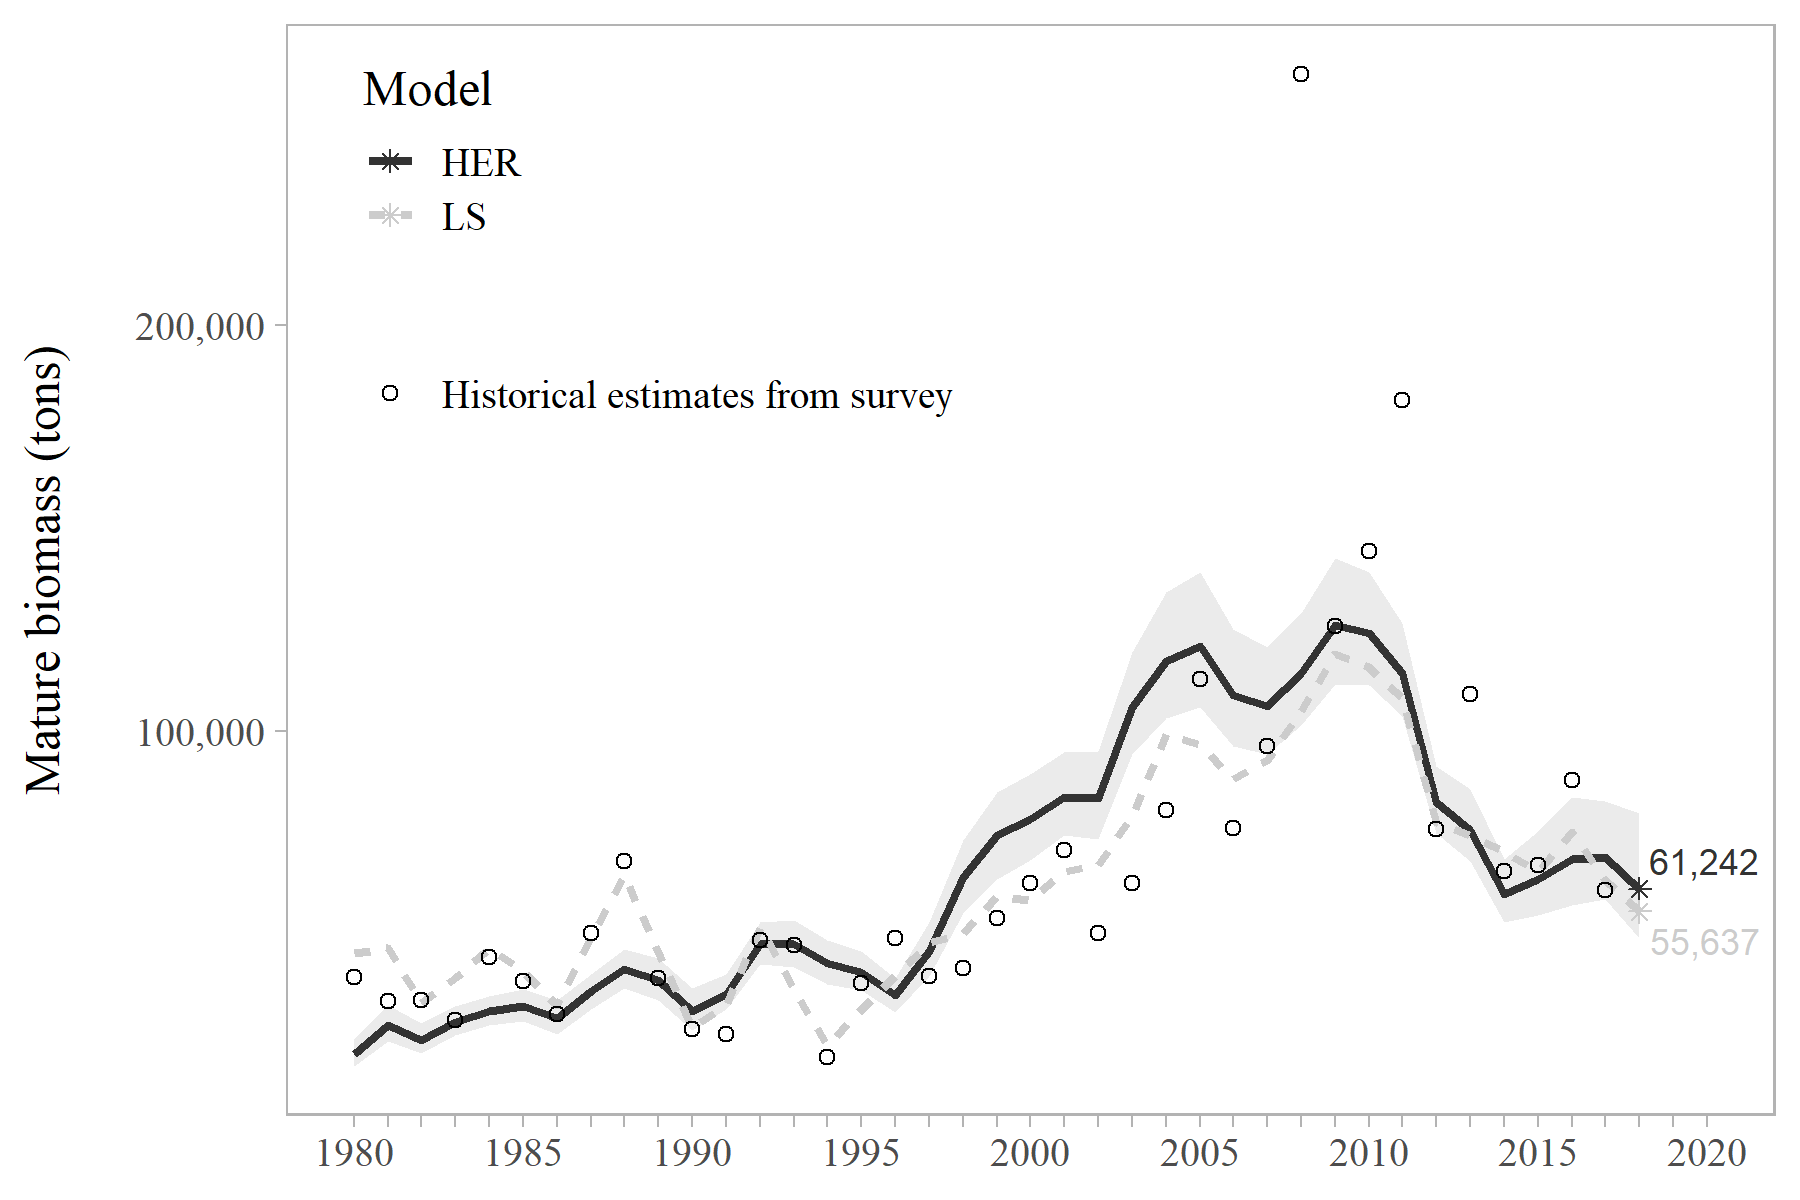
\includegraphics[width=1\linewidth]{../../HER/figs/compare_matbiomass}

Figure 2. Model-estimated mature biomass in HER (black solid line) and
LS (grey dashed line) compared to historical estimates from the survey
(open circles) that convert survey egg deposition to biomass using
catch, age composition, and weight-at-age data. The asterix (*) and
corresponding labels show the forecasted mature biomass for each model.
The shaded region around the HER fit is the 95\% credibility interval.

Although it is not a comparison of HER and LS, we revamped the figure
code for the LS comparison of past assessment models' estimates and
forecasts of mature biomass (Figure 3).

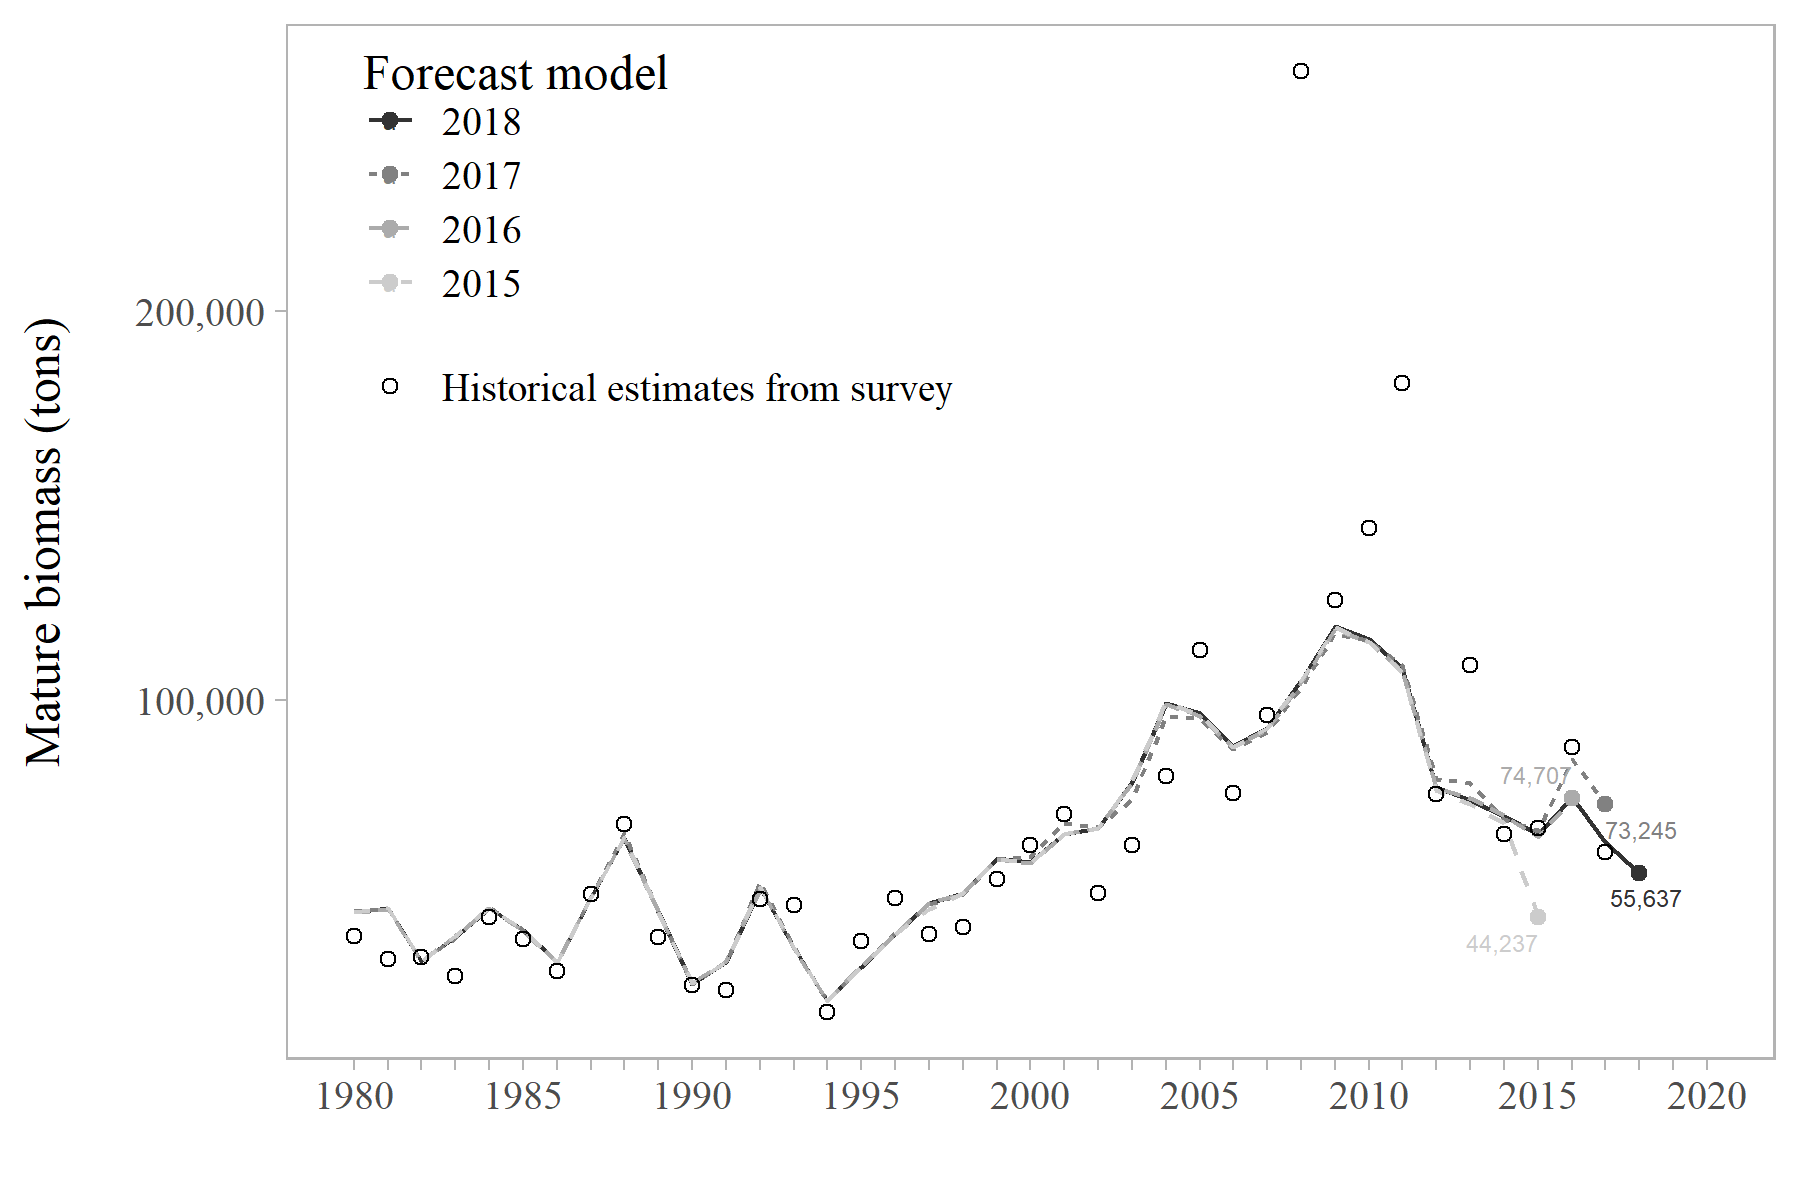
\includegraphics[width=1\linewidth]{../../HER/figs/LS/compare_past_matbio}

Figure 3. Model-estimated mature biomass from the ``, YEAR,'' and
previous three forecast models compared to historical estimates from the
survey (open circles) that convert survey egg deposition to mature
biomass using catch, age composition, and weight-at-age data. To aid in
visualization, the older the estimate/forecast, the lighter the color.

Similarly, we also revamped the figure code for comparing catch/GHL and
spawing biomass for the LS model (Figure 4)

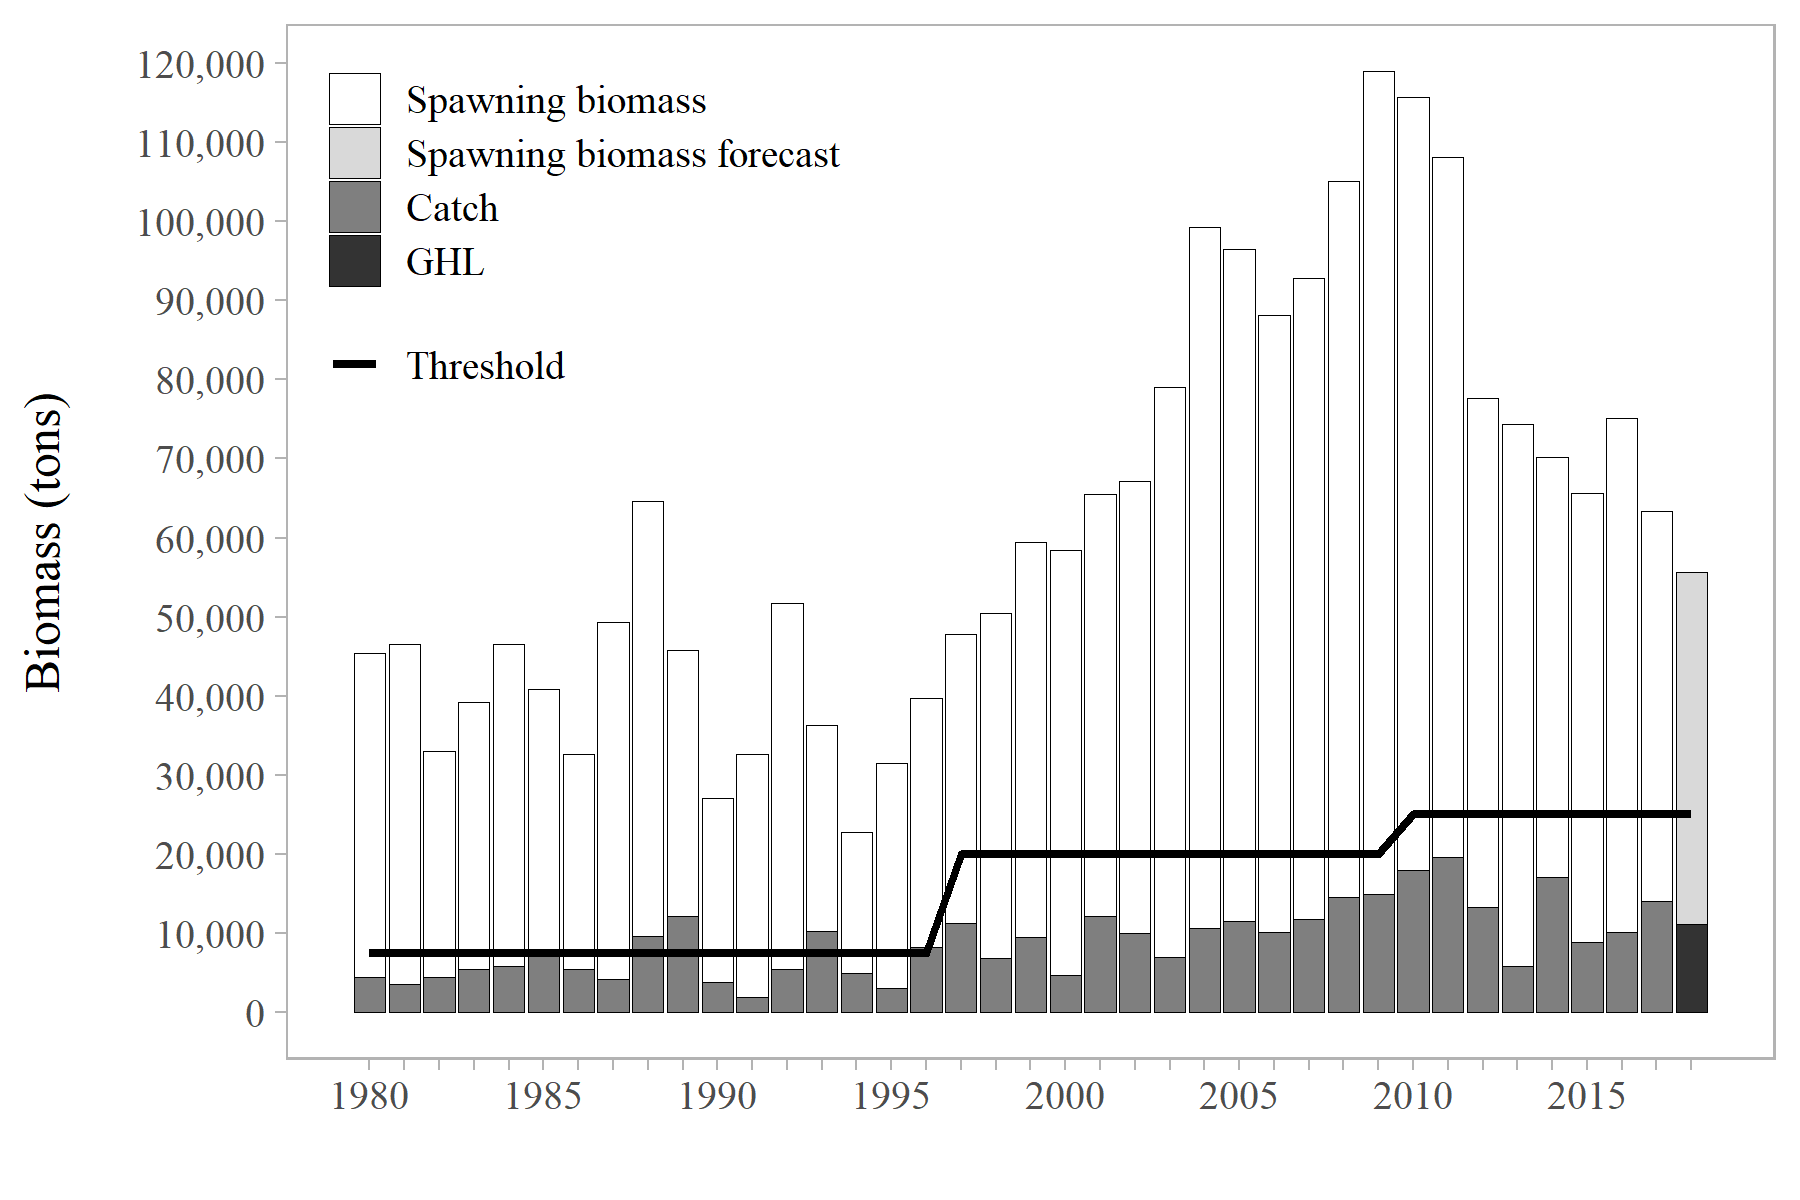
\includegraphics{../../HER/figs/LS/biomasscatch_barplot.png}

Figure 4. Stacked bar graph of spawning biomass (white), spawning
biomass forecast (light grey), catch (dark grey), and the GHL (black).
The threshold (black line) is the biomass level defined in regulation
below which no fishery occurs. The harvest (or GHL) plus the spawning
biomass equals the mature biomass. If there is no catch (or GHL), the
spawning biomass (or spawning biomass forecast) equals the mature
biomass (or mature biomass forecast).

\subsection{Egg deposition}\label{egg-deposition}

The HER and LS model track the historical survey estimates of egg
deposition reasonably well in terms of magnitude and trend (Figure 5),
although the LS model fits considerably better. The HER model shows a
strong residual pattern, starting with all positive residuals and
switching to all negative residuals (Figure 6), which in demonstrative
of poor fit.

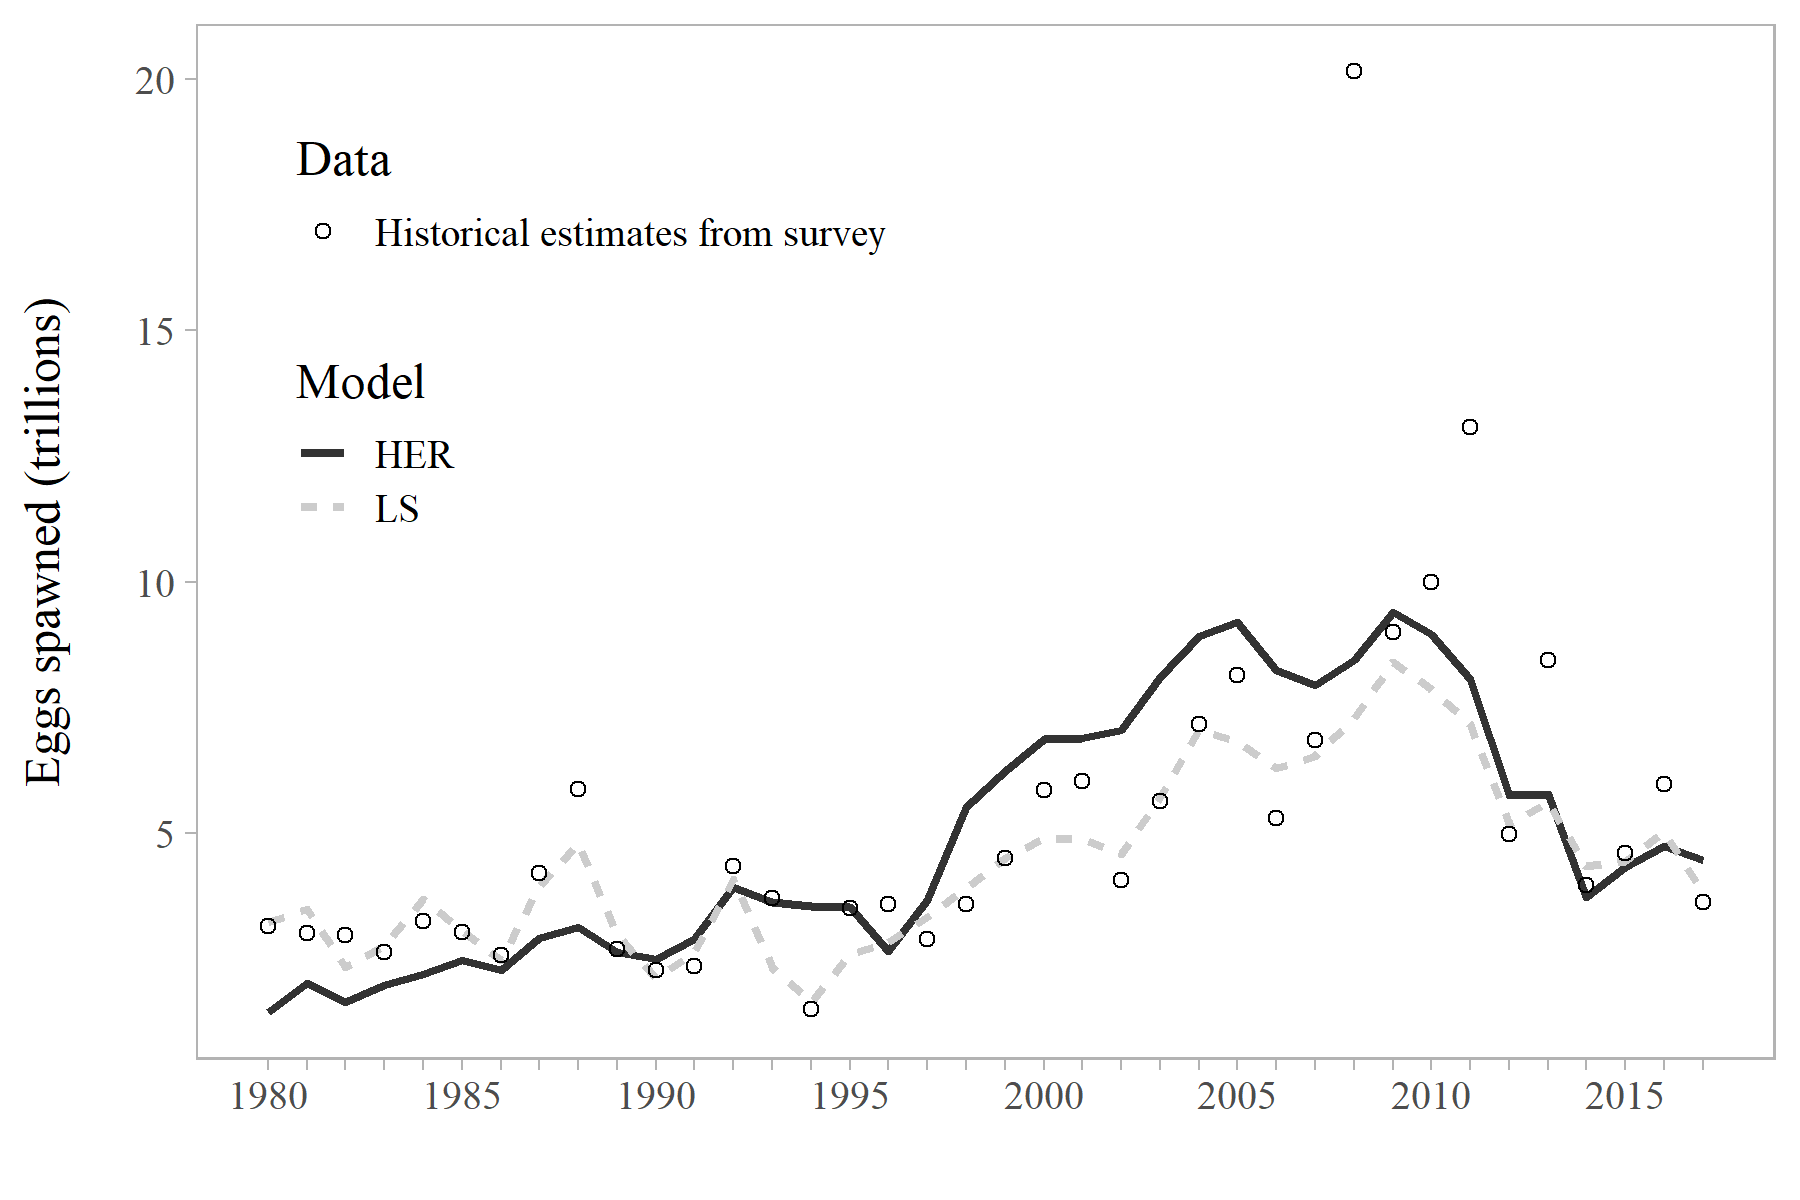
\includegraphics[width=1\linewidth]{../../HER/figs/compare_eggdep_plot}

Figure 5. Model-estimated egg deposition (number of eggs spawned in
trillions) in HER (black solid line) and LS (grey dashed line) compared
to historical estimates from the survey (open circles). The grey bars
show the boostrap-estimated 95\% confidence interval for the survey
estimates.

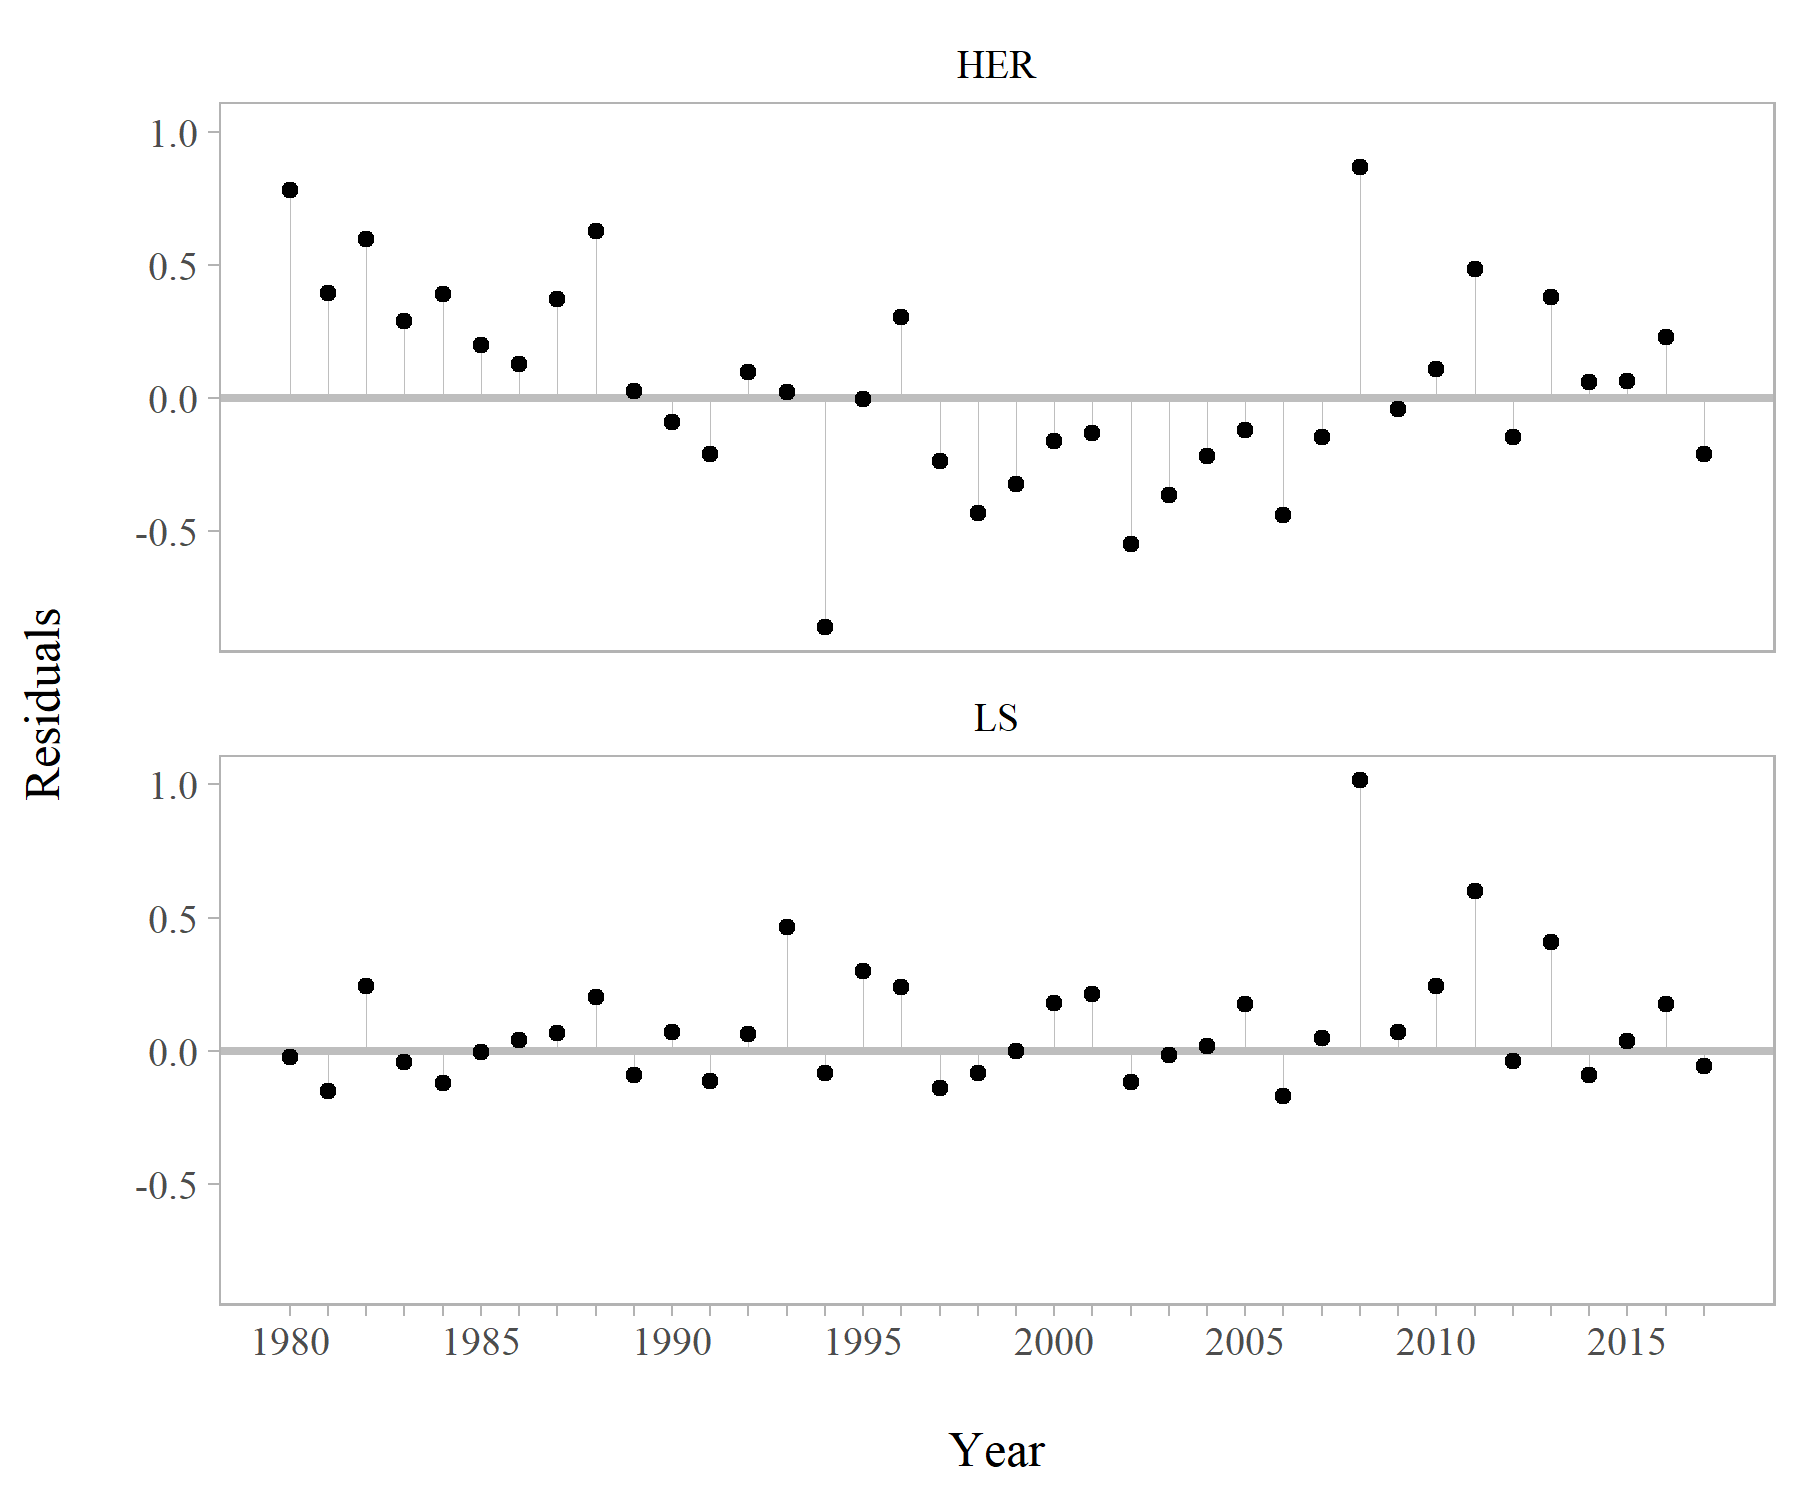
\includegraphics[width=1\linewidth]{../../HER/figs/compare_eggresids}

Figure 6. A comparison of HER (top panel) and LS (bottom panel) egg
deposition residuals calculated as the difference between survey and
model-estimated egg deposition on the logarithmic scale.

\section{Age Compositions}\label{age-compositions}

\subsection{Composition data}\label{composition-data}

New figures for commercial catch and cast net survey age compositions
for Sitka have been created for this project (Figure 7).

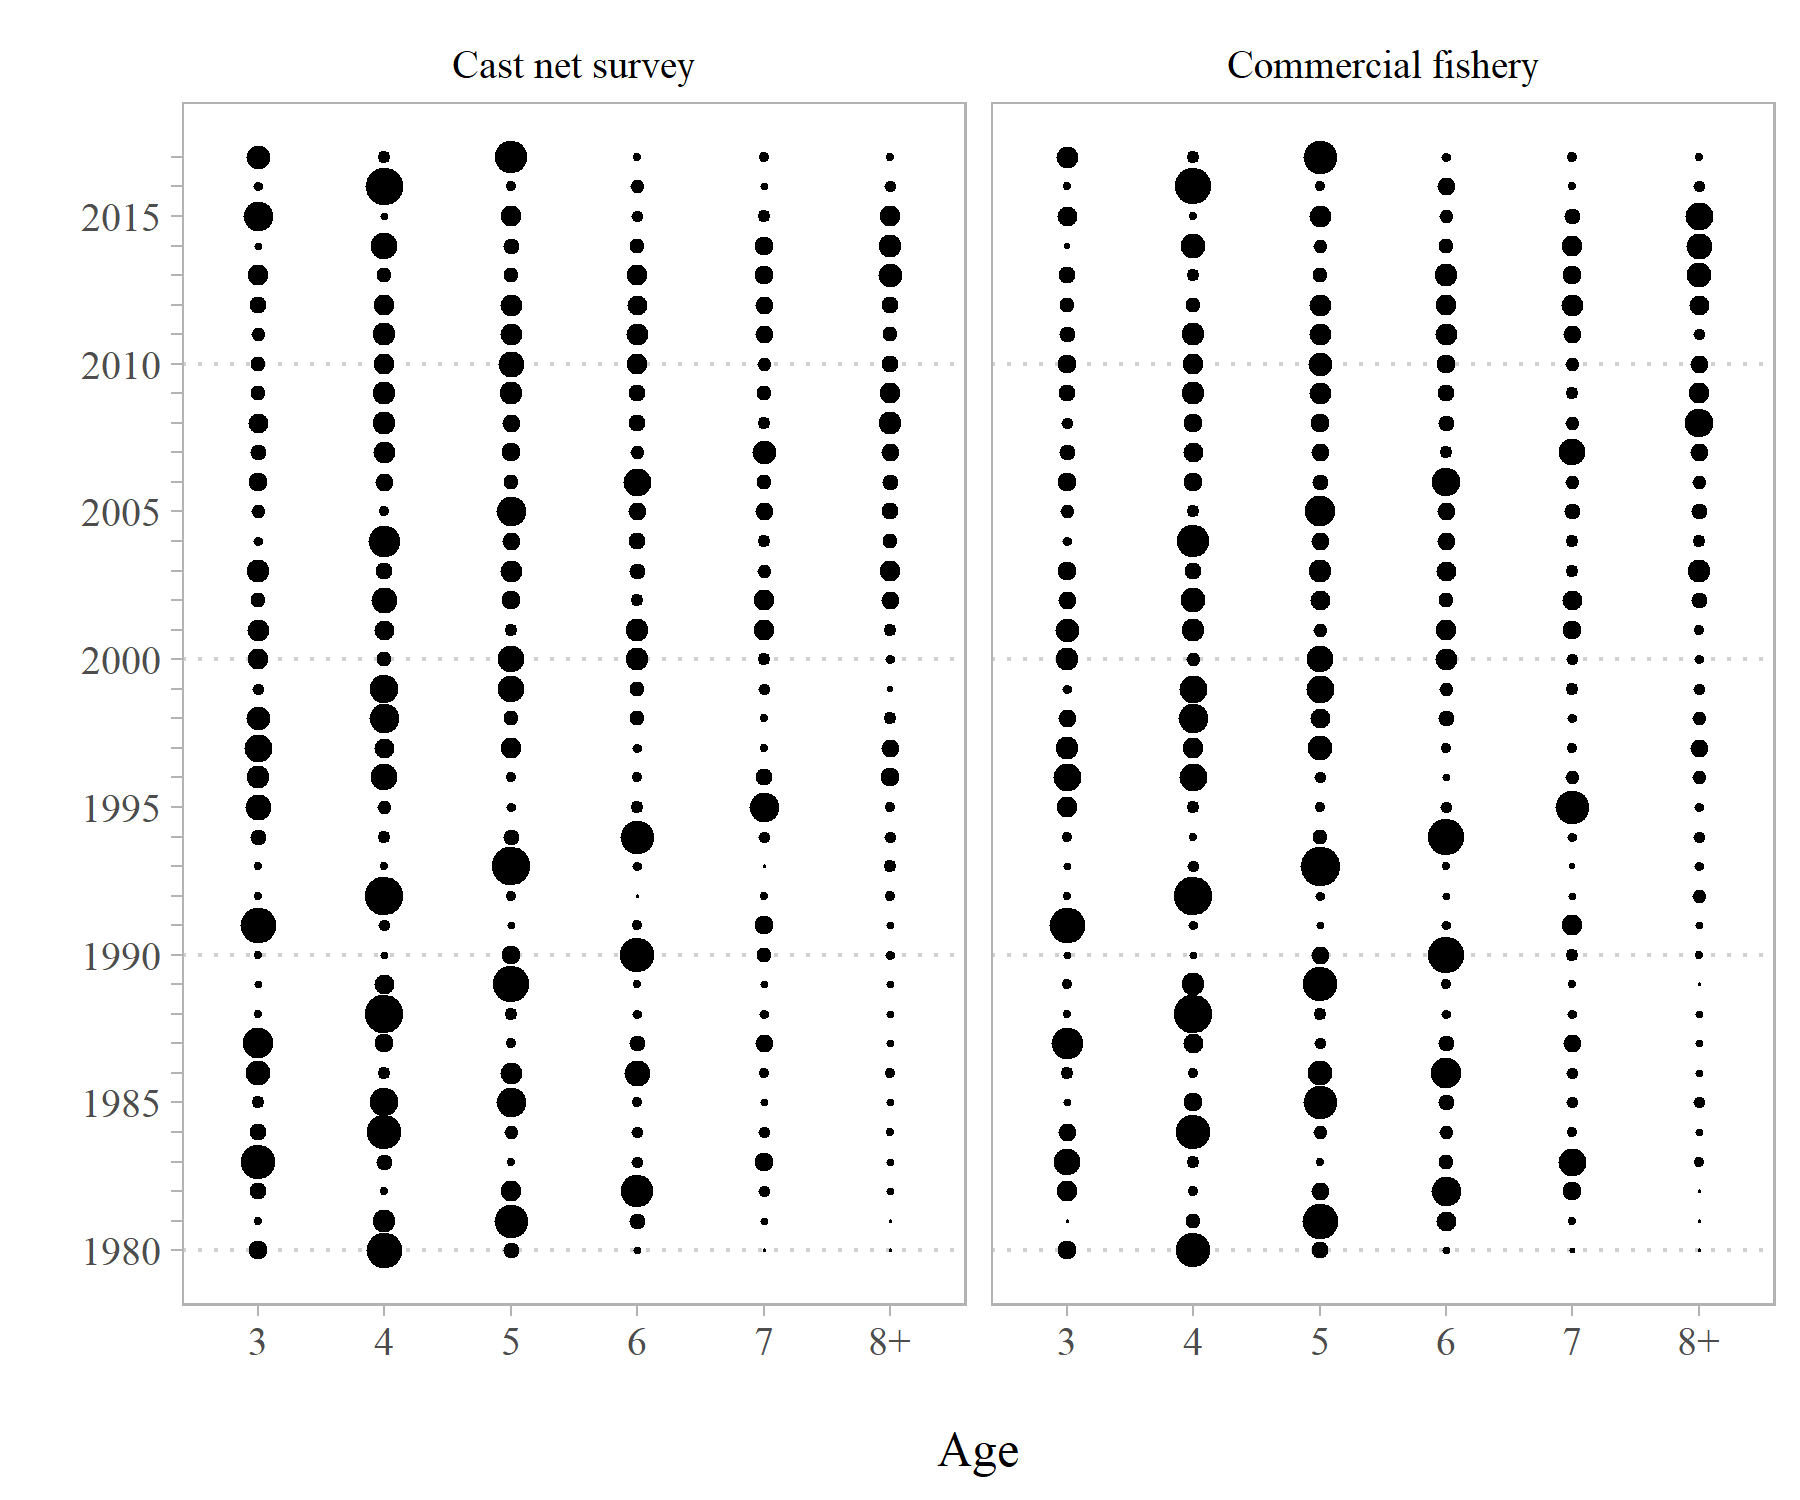
\includegraphics[width=1\linewidth]{../../HER/figs/HER/agecomps_bubbleplot}

Figure 7. Cast net survey (left panel) and commercial seine fishery
(right panel) age compositions by year.

\subsection{Residuals}\label{residuals}

The HER model shows a moderate residual pattern in both age composition
data sources in ages-7 and 8+, switching from predominately negative
residuals around 1998 (Figure 8). The LS model does not show this strong
of pattern (Figure 9).

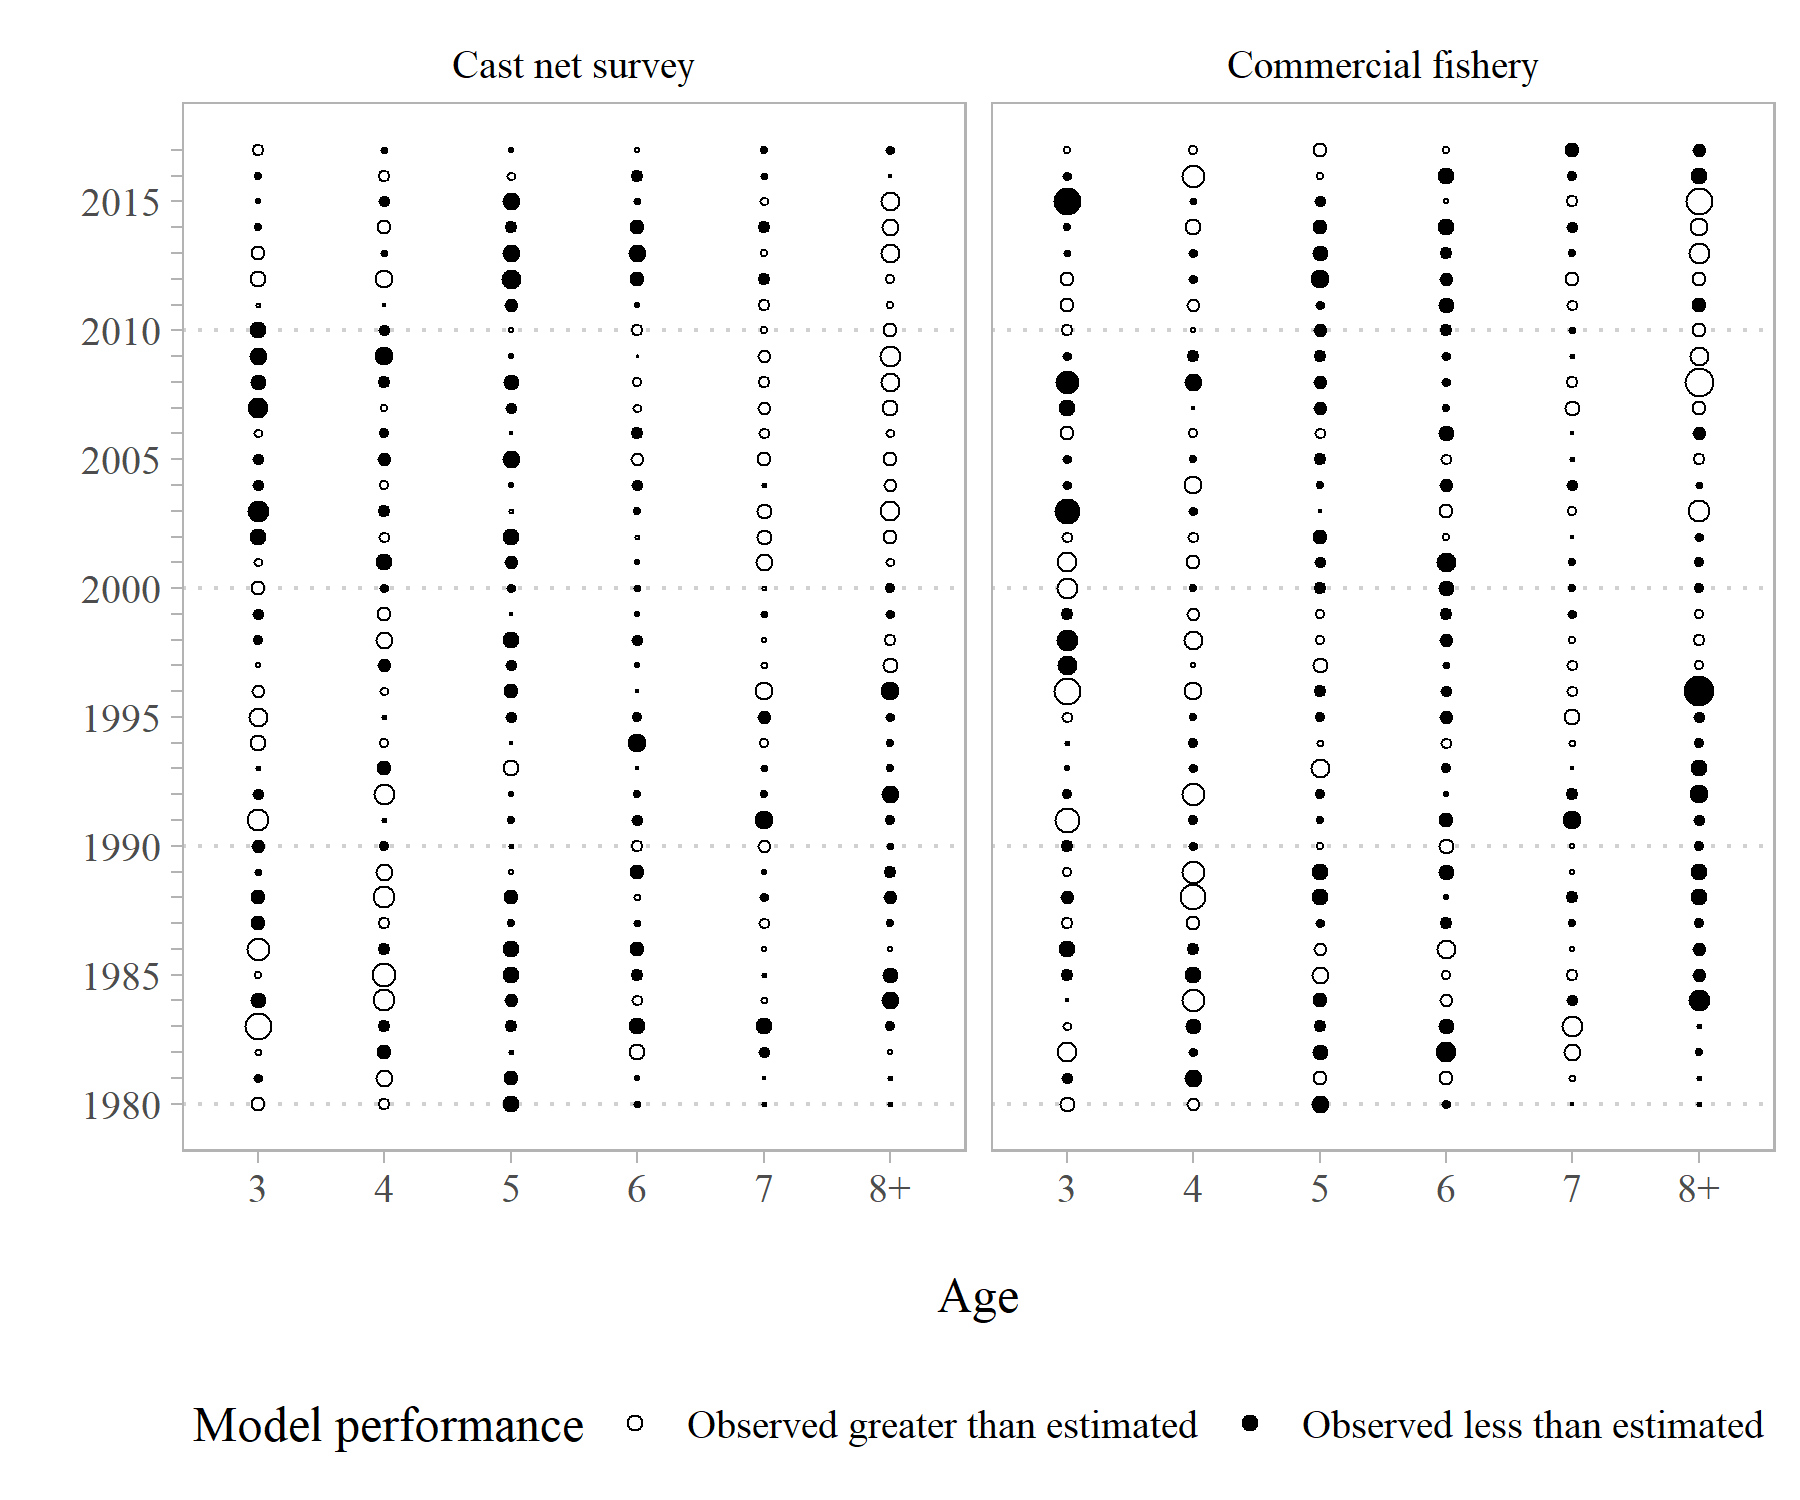
\includegraphics[width=1\linewidth]{../../HER/figs/HER/HER_agecomps_residplot}

Figure 8. Cast net survey (left panel) and commercial seine fishery
(right panel) age composition residuals for the HER model, calculated as
the difference between observed proportion-at-age and estimated
proportion-at-age.. A positive residual (white) indicates that the
observed value is greater than the model estimate, and negative (black)
means the opposite. The size of the circle is relative to the size of
the residual.

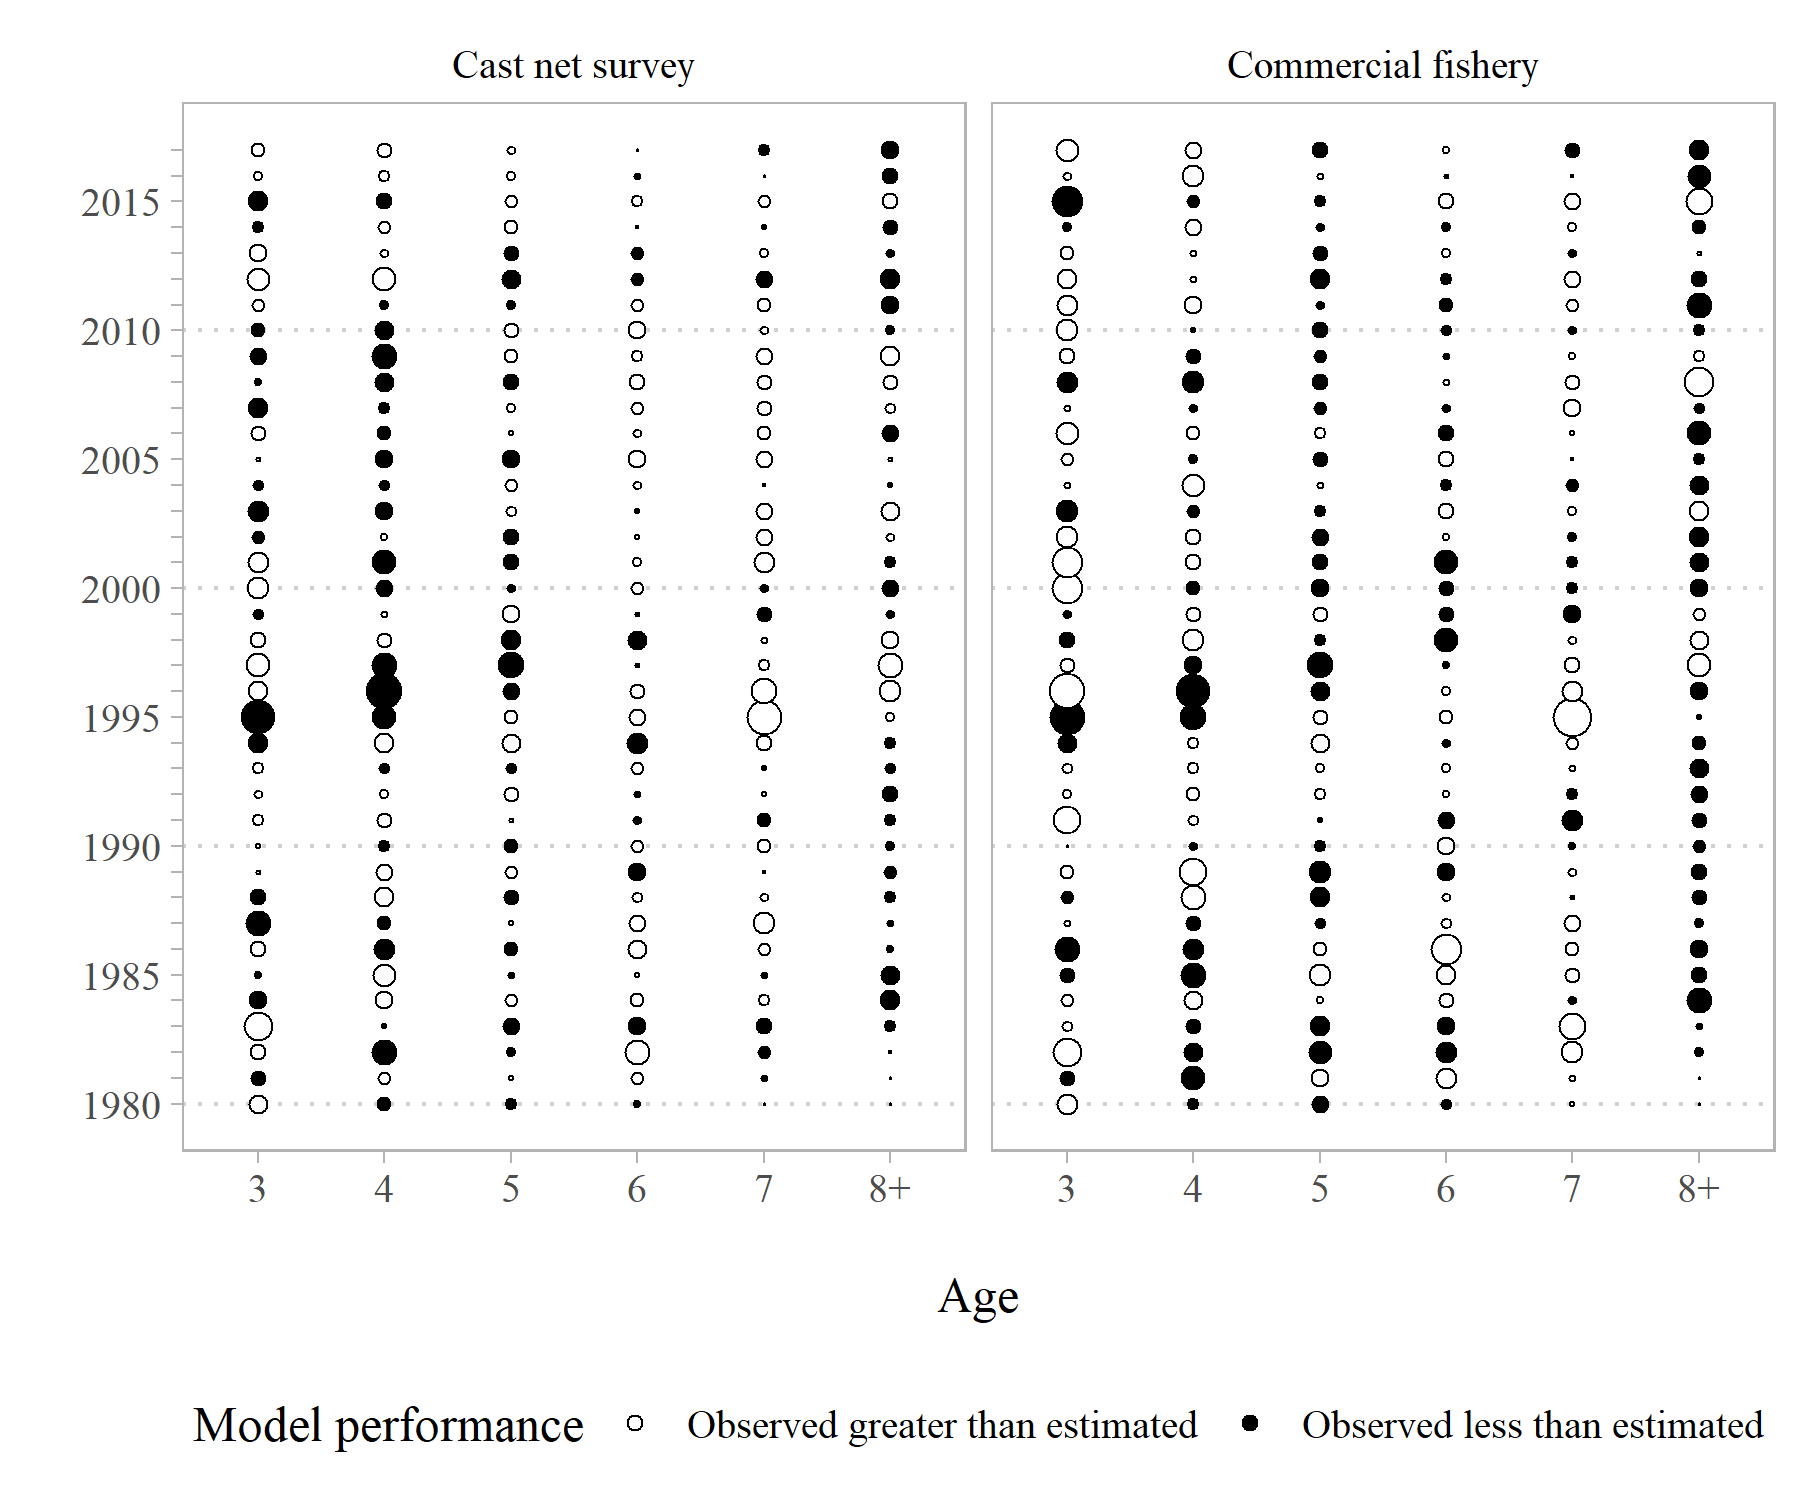
\includegraphics[width=1\linewidth]{../../HER/figs/LS/LS_agecomps_residplot}

Figure 9. Cast net survey (left panel) and commercial seine fishery
(right panel) age composition residuals for the LS model, calculated as
the difference between observed proportion-at-age and estimated
proportion-at-age. A positive residual (white) indicates that the
observed value is greater than the model estimate, and negative (black)
means the opposite. The size of the circle is relative to the size of
the residual.

\subsection{Comparison of fits}\label{comparison-of-fits}

Despite the residual pattern in HER, both models fit the catch (Figure
10) and cast net (Figure 11) age composition data well.

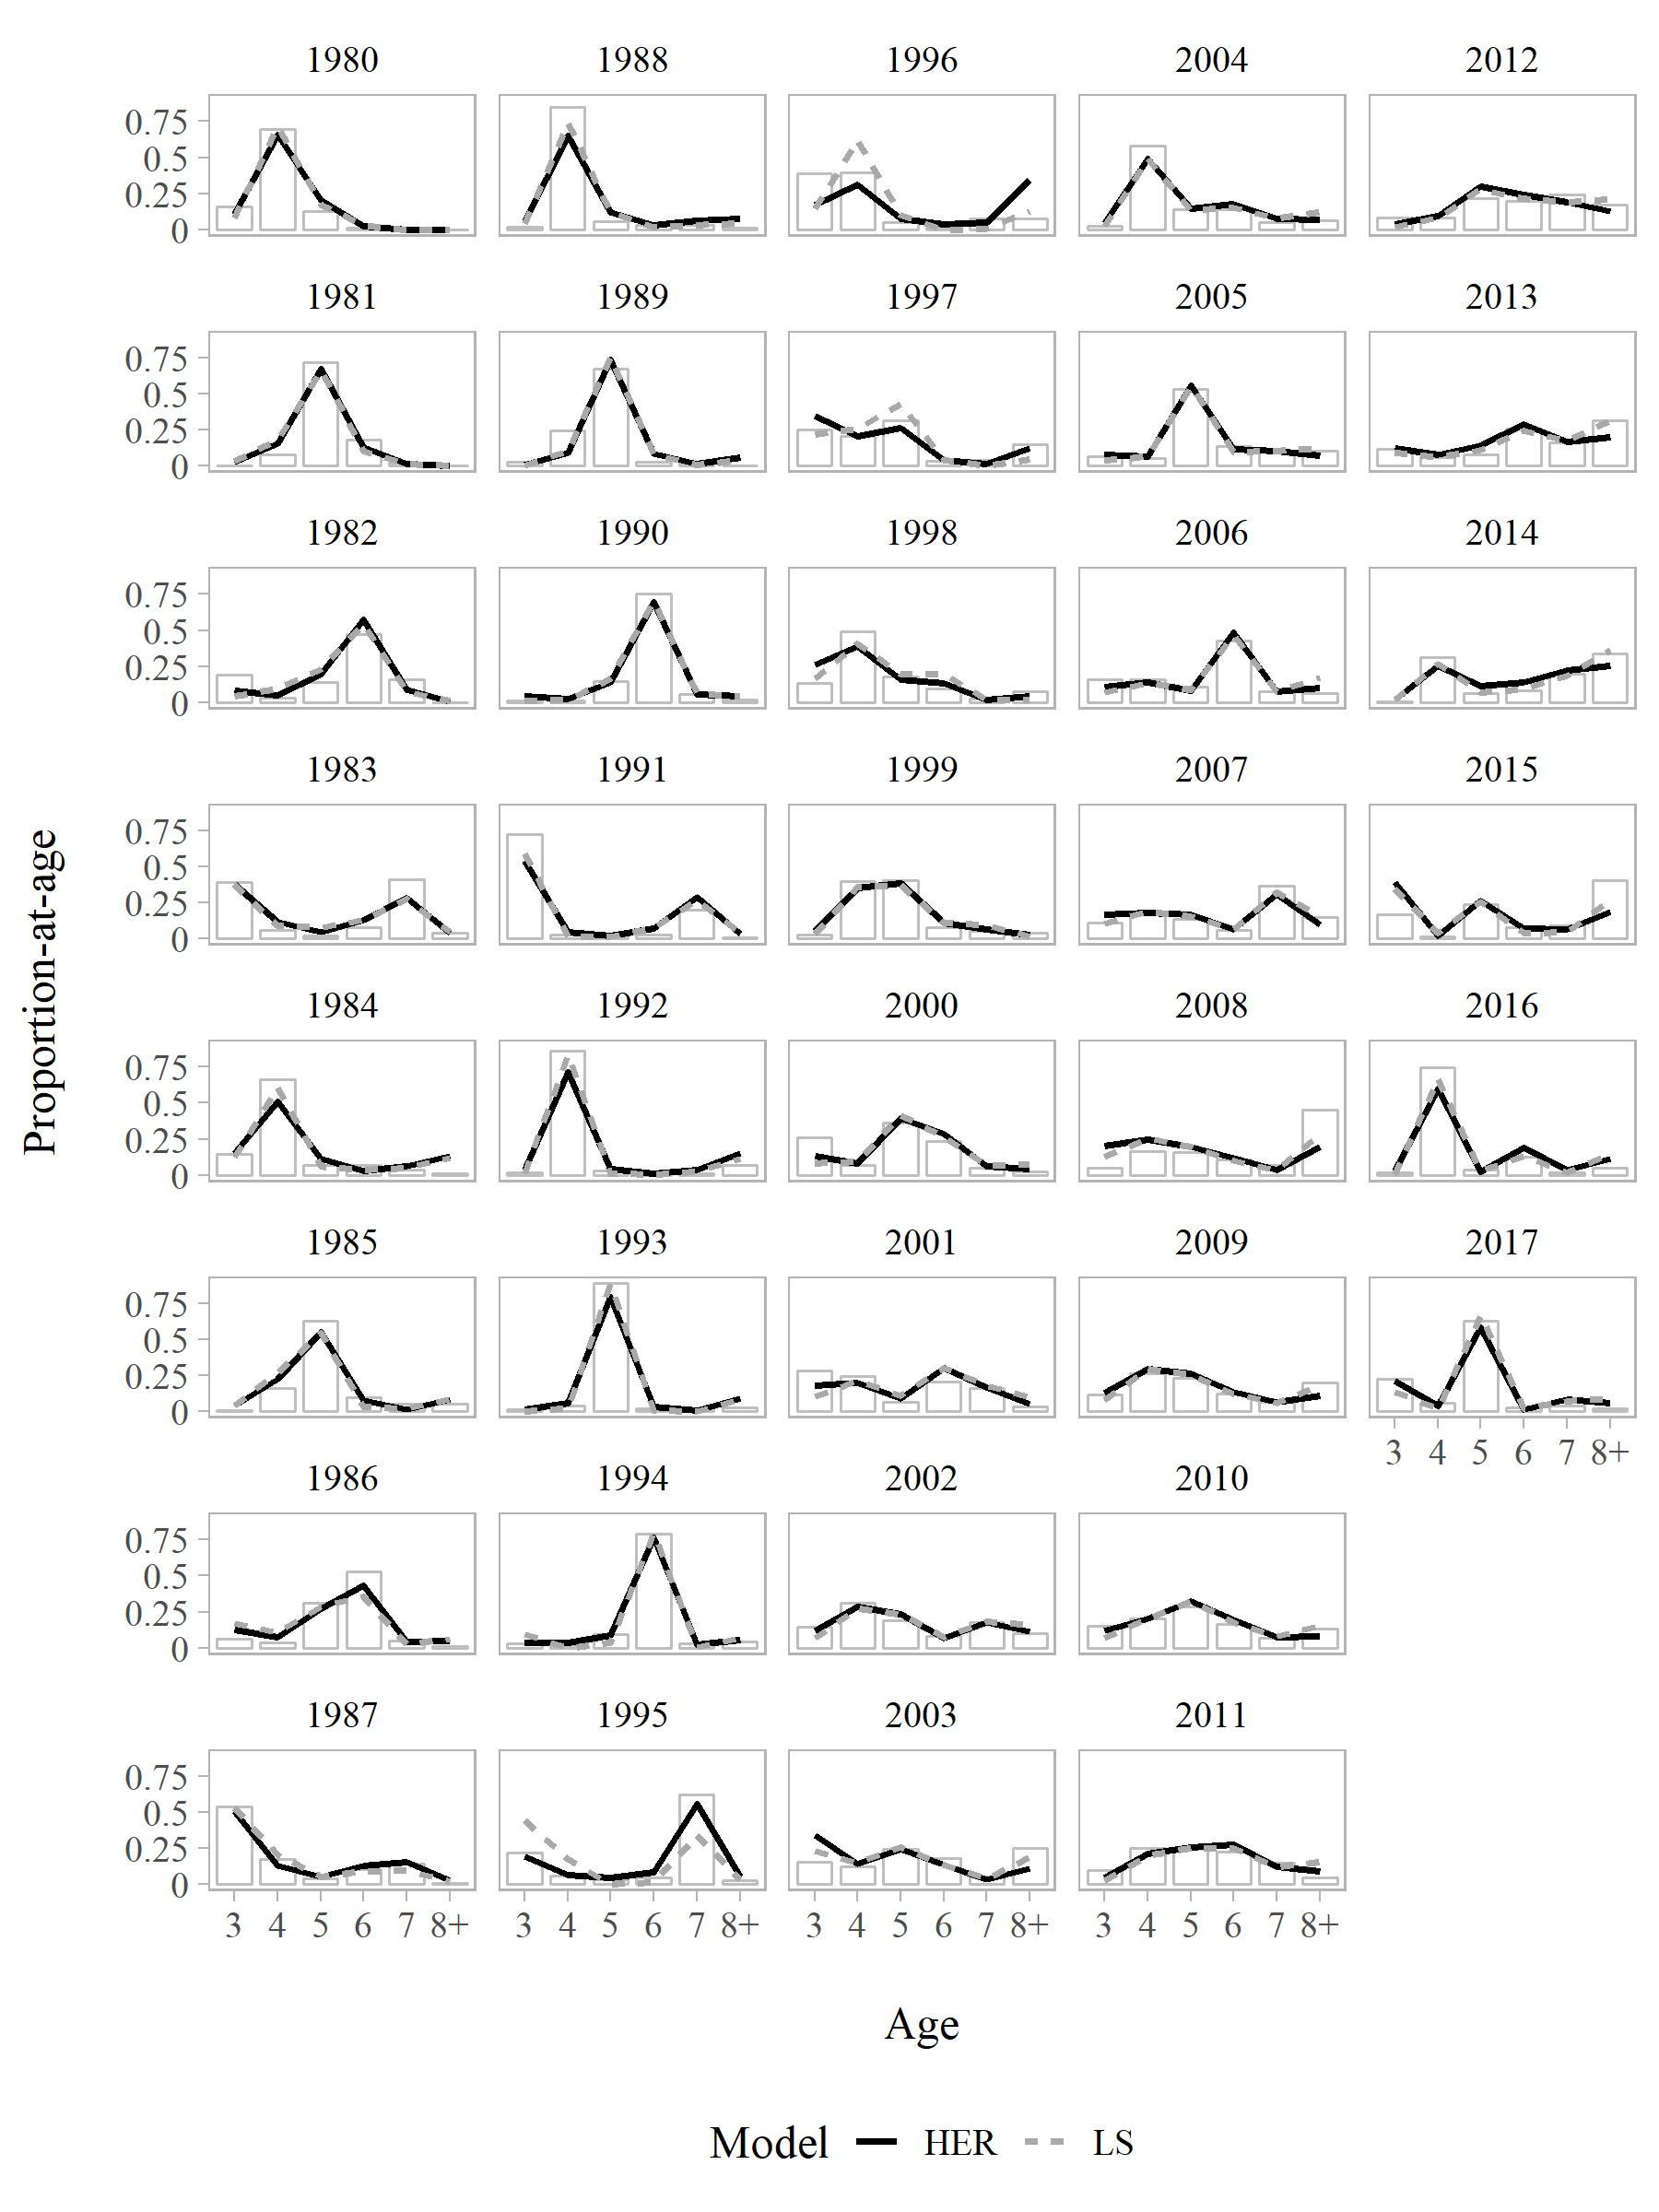
\includegraphics[width=1\linewidth]{../../HER/figs/compare_catchcomp_barplot}

Figure 10. Proportion-at-age observed in the commercial seine fishery
(white bars) compared to model-estimated proportion-at-age in HER (black
solid lines) and LS (grey dashed lines).

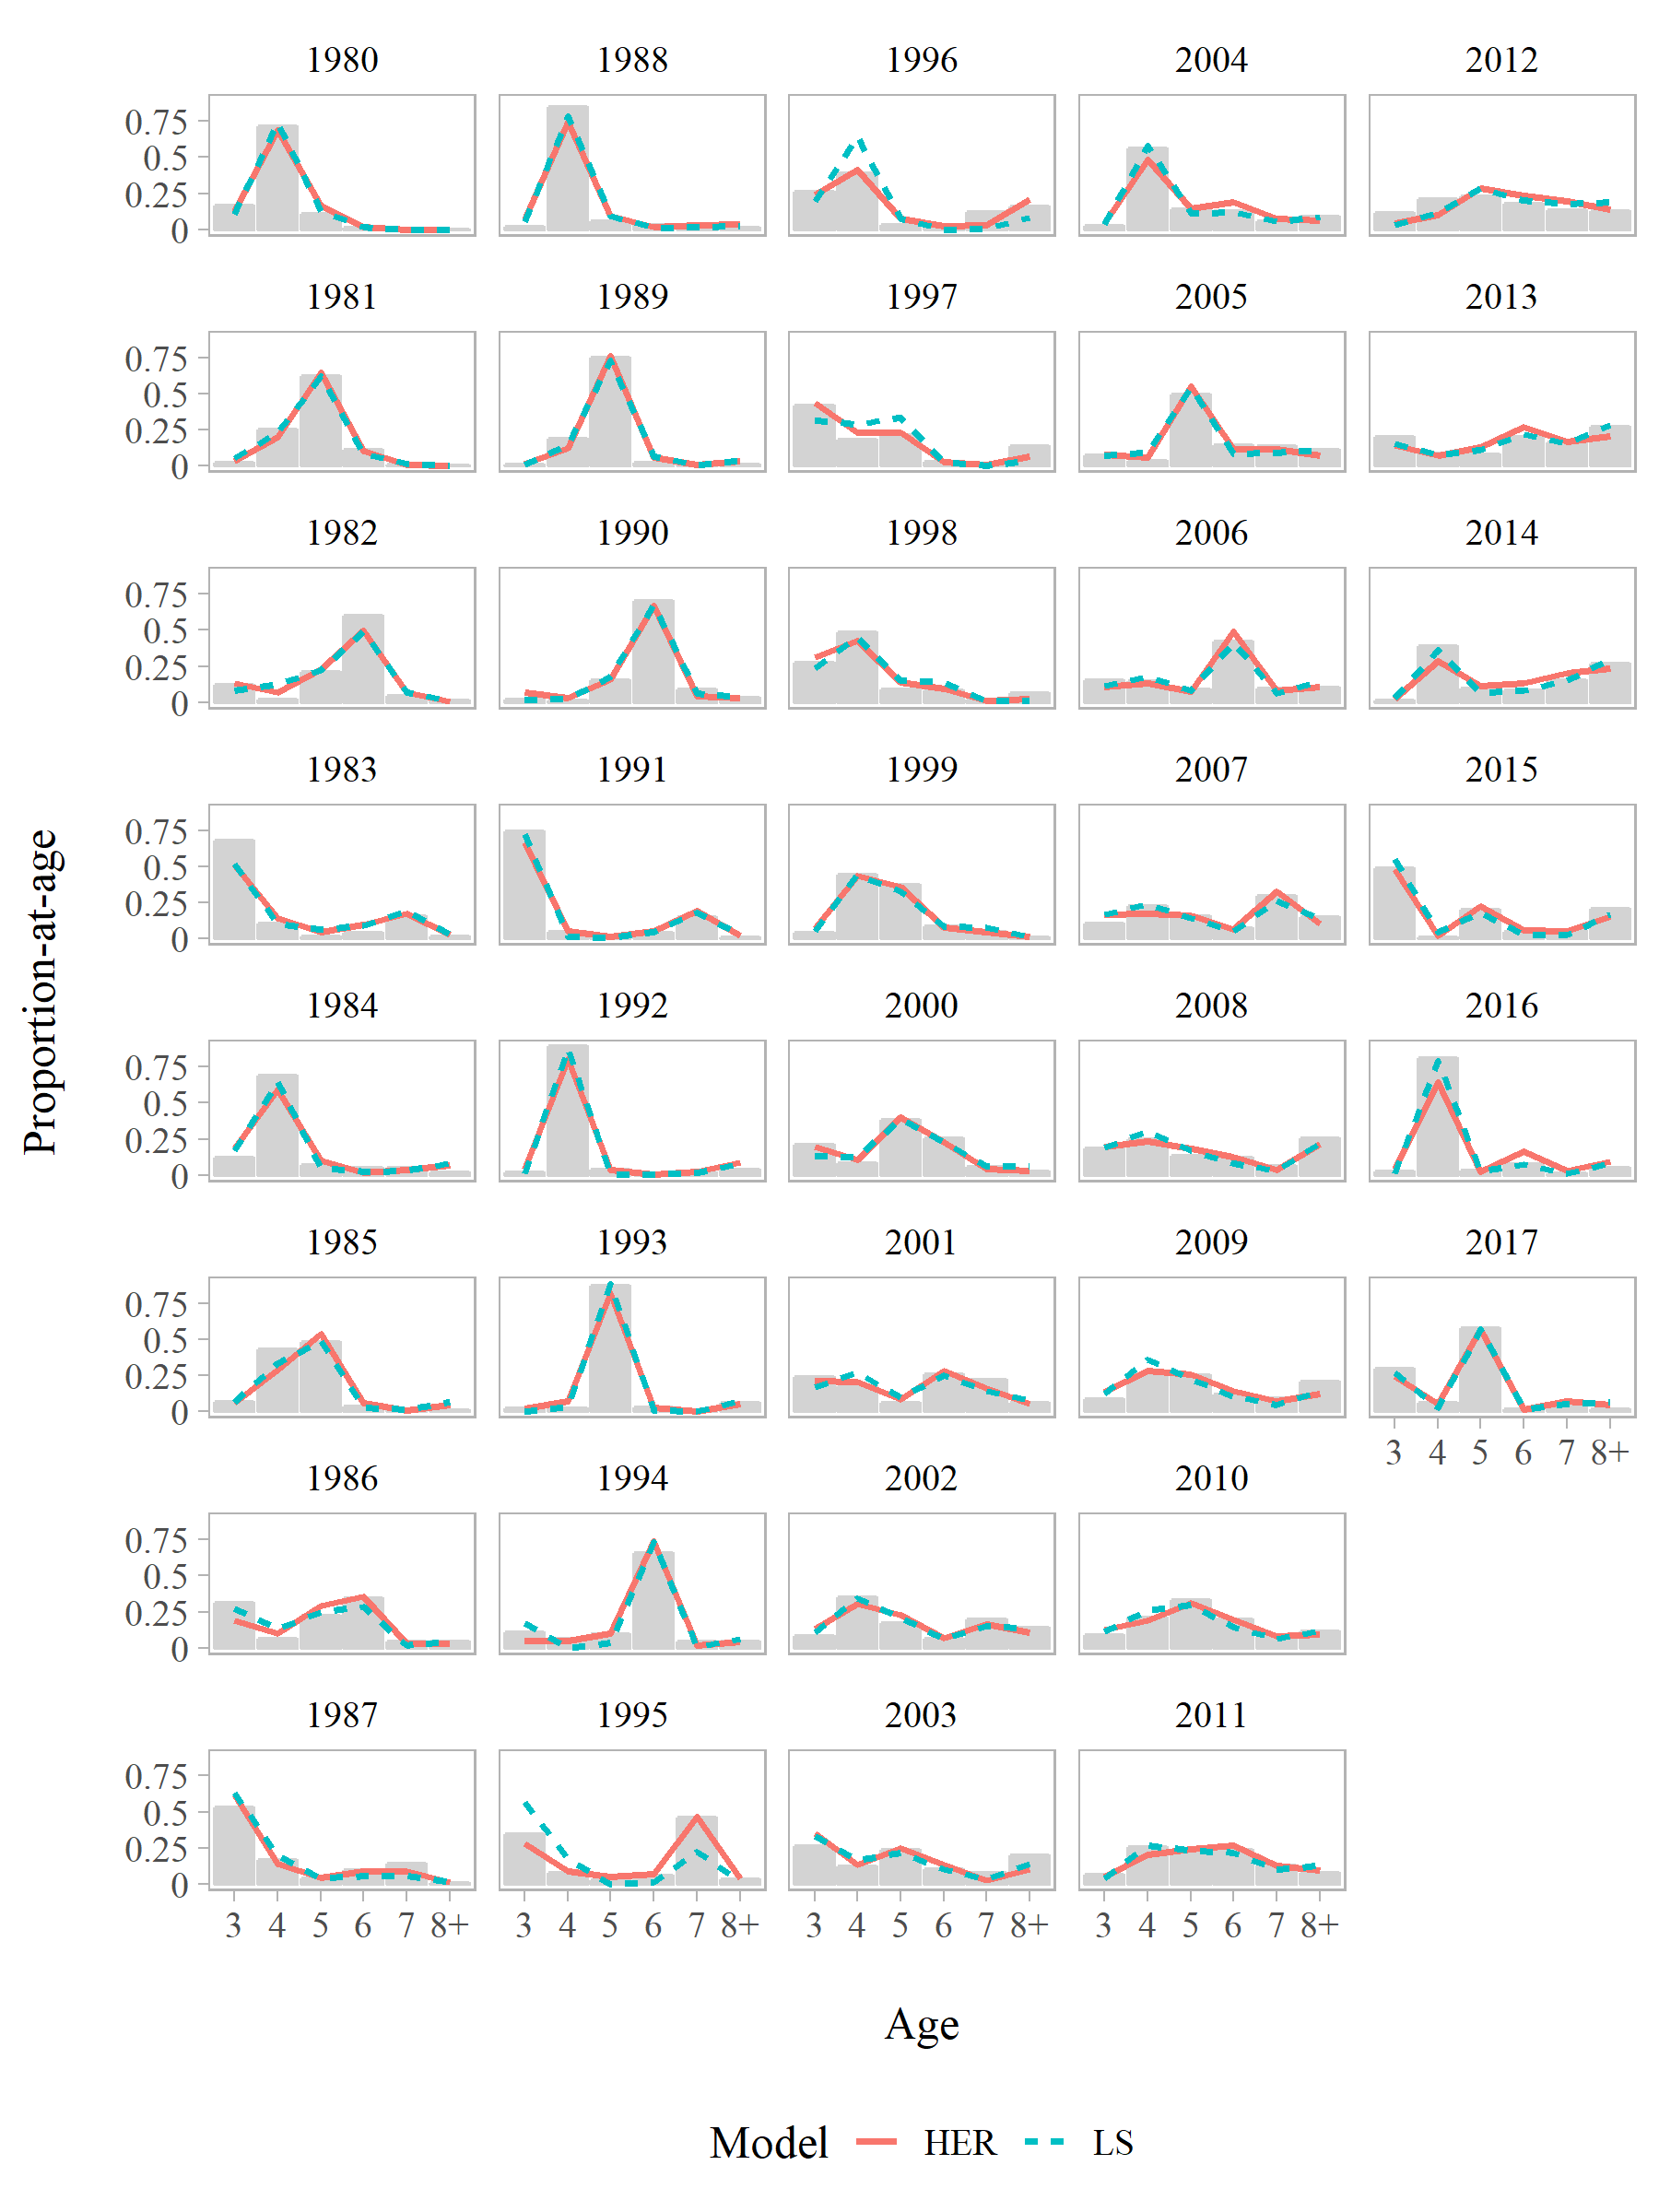
\includegraphics[width=1\linewidth]{../../HER/figs/compare_spcomp_barplot}

Figure 11. Proportion-at-age observed in the cast net survey (white
bars) compared to model-estimated proportion-at-age in HER (black solid
lines) and LS (grey dashed lines).

\section{Recruitment}\label{recruitment}

Although the trends in recruitment are similar between HER and LS, the
magntitude is quite different (Figure 12 and Figure 13). We attribute
this difference to the manual weighting of the LS stock-recruitment
relationship to zero, whereas HER appears to put a stronger weighting on
this relationship. Neither model shows a concerning residual trend
(Figure 14).

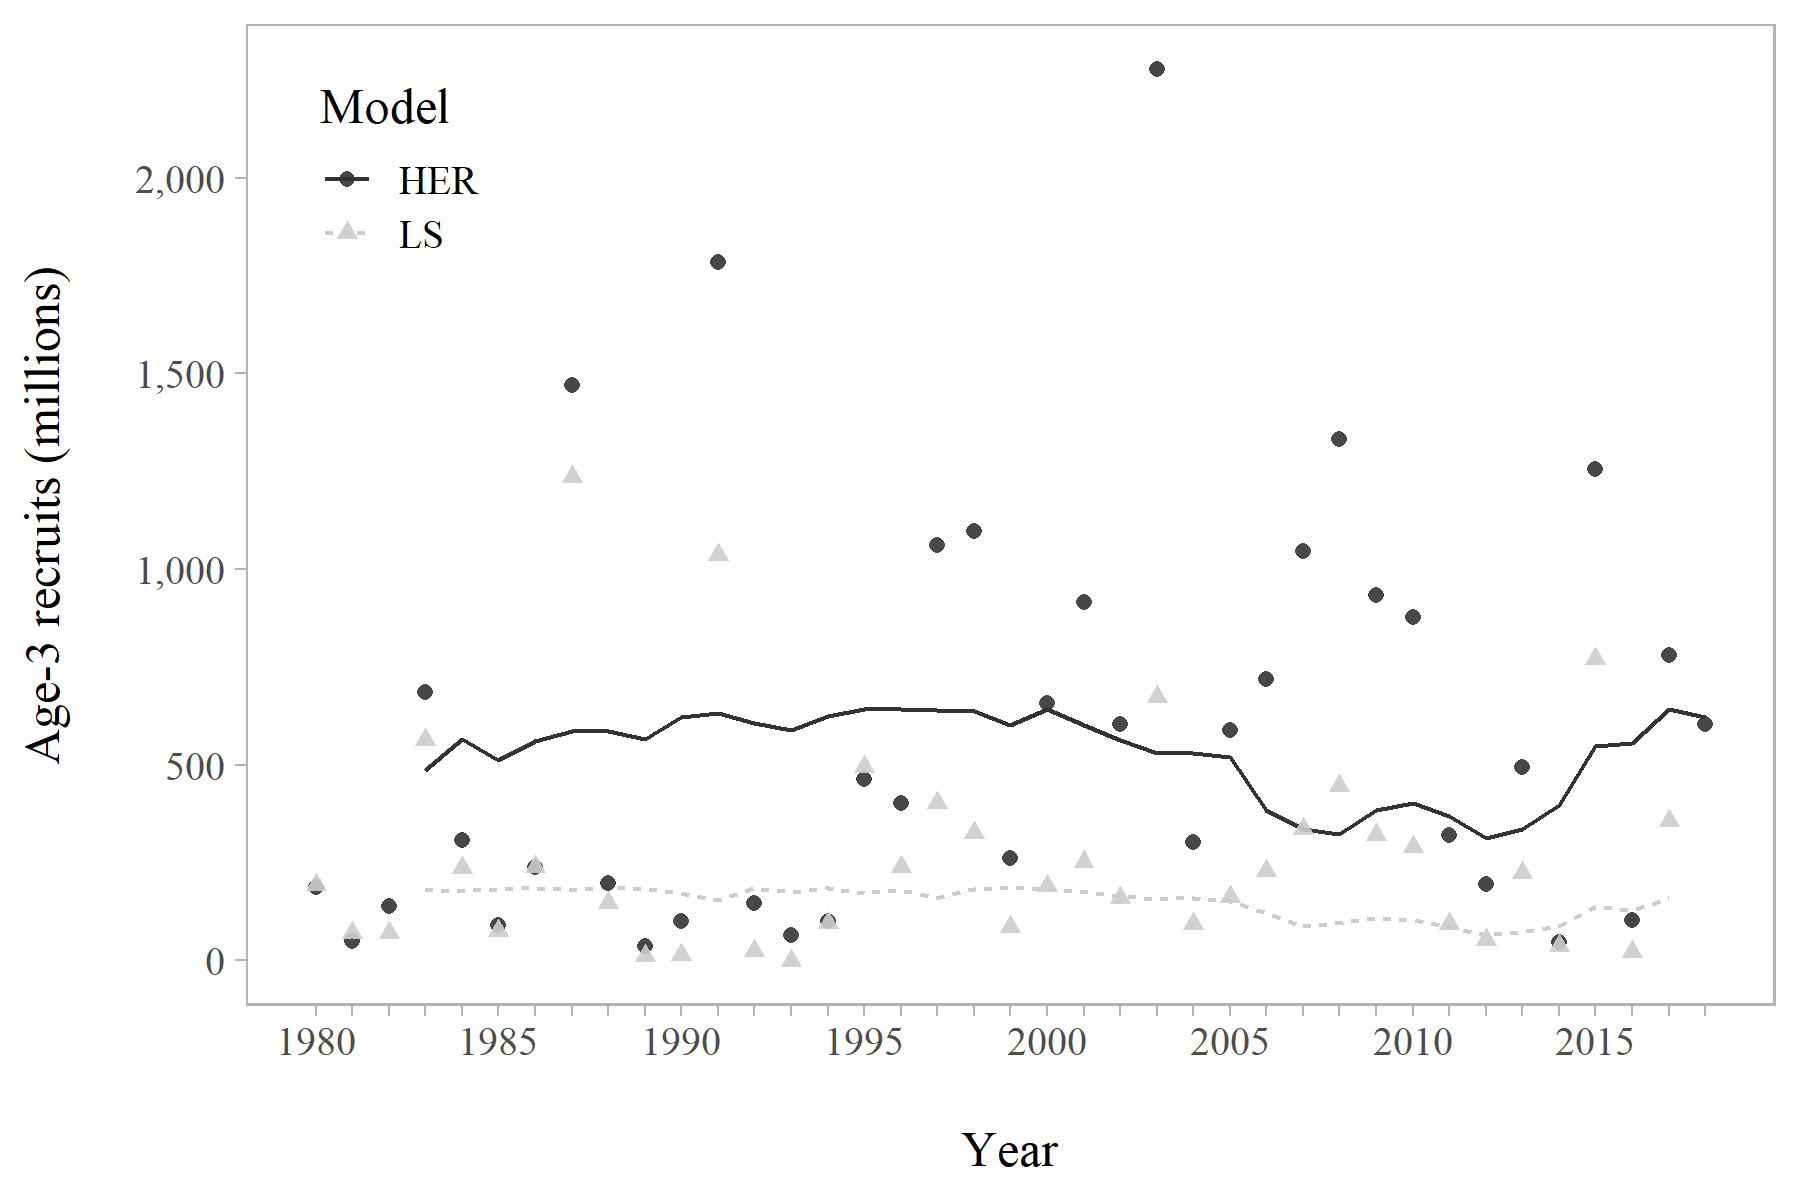
\includegraphics[width=1\linewidth]{../../HER/figs/compare_recruit_plot}

Figure 12. A comparison of estimated age-3 recruits in millions from the
Ricker model (lines) and age-structured model (points) in HER (black
solid line and circles) and LS (grey dashed line and triangles).

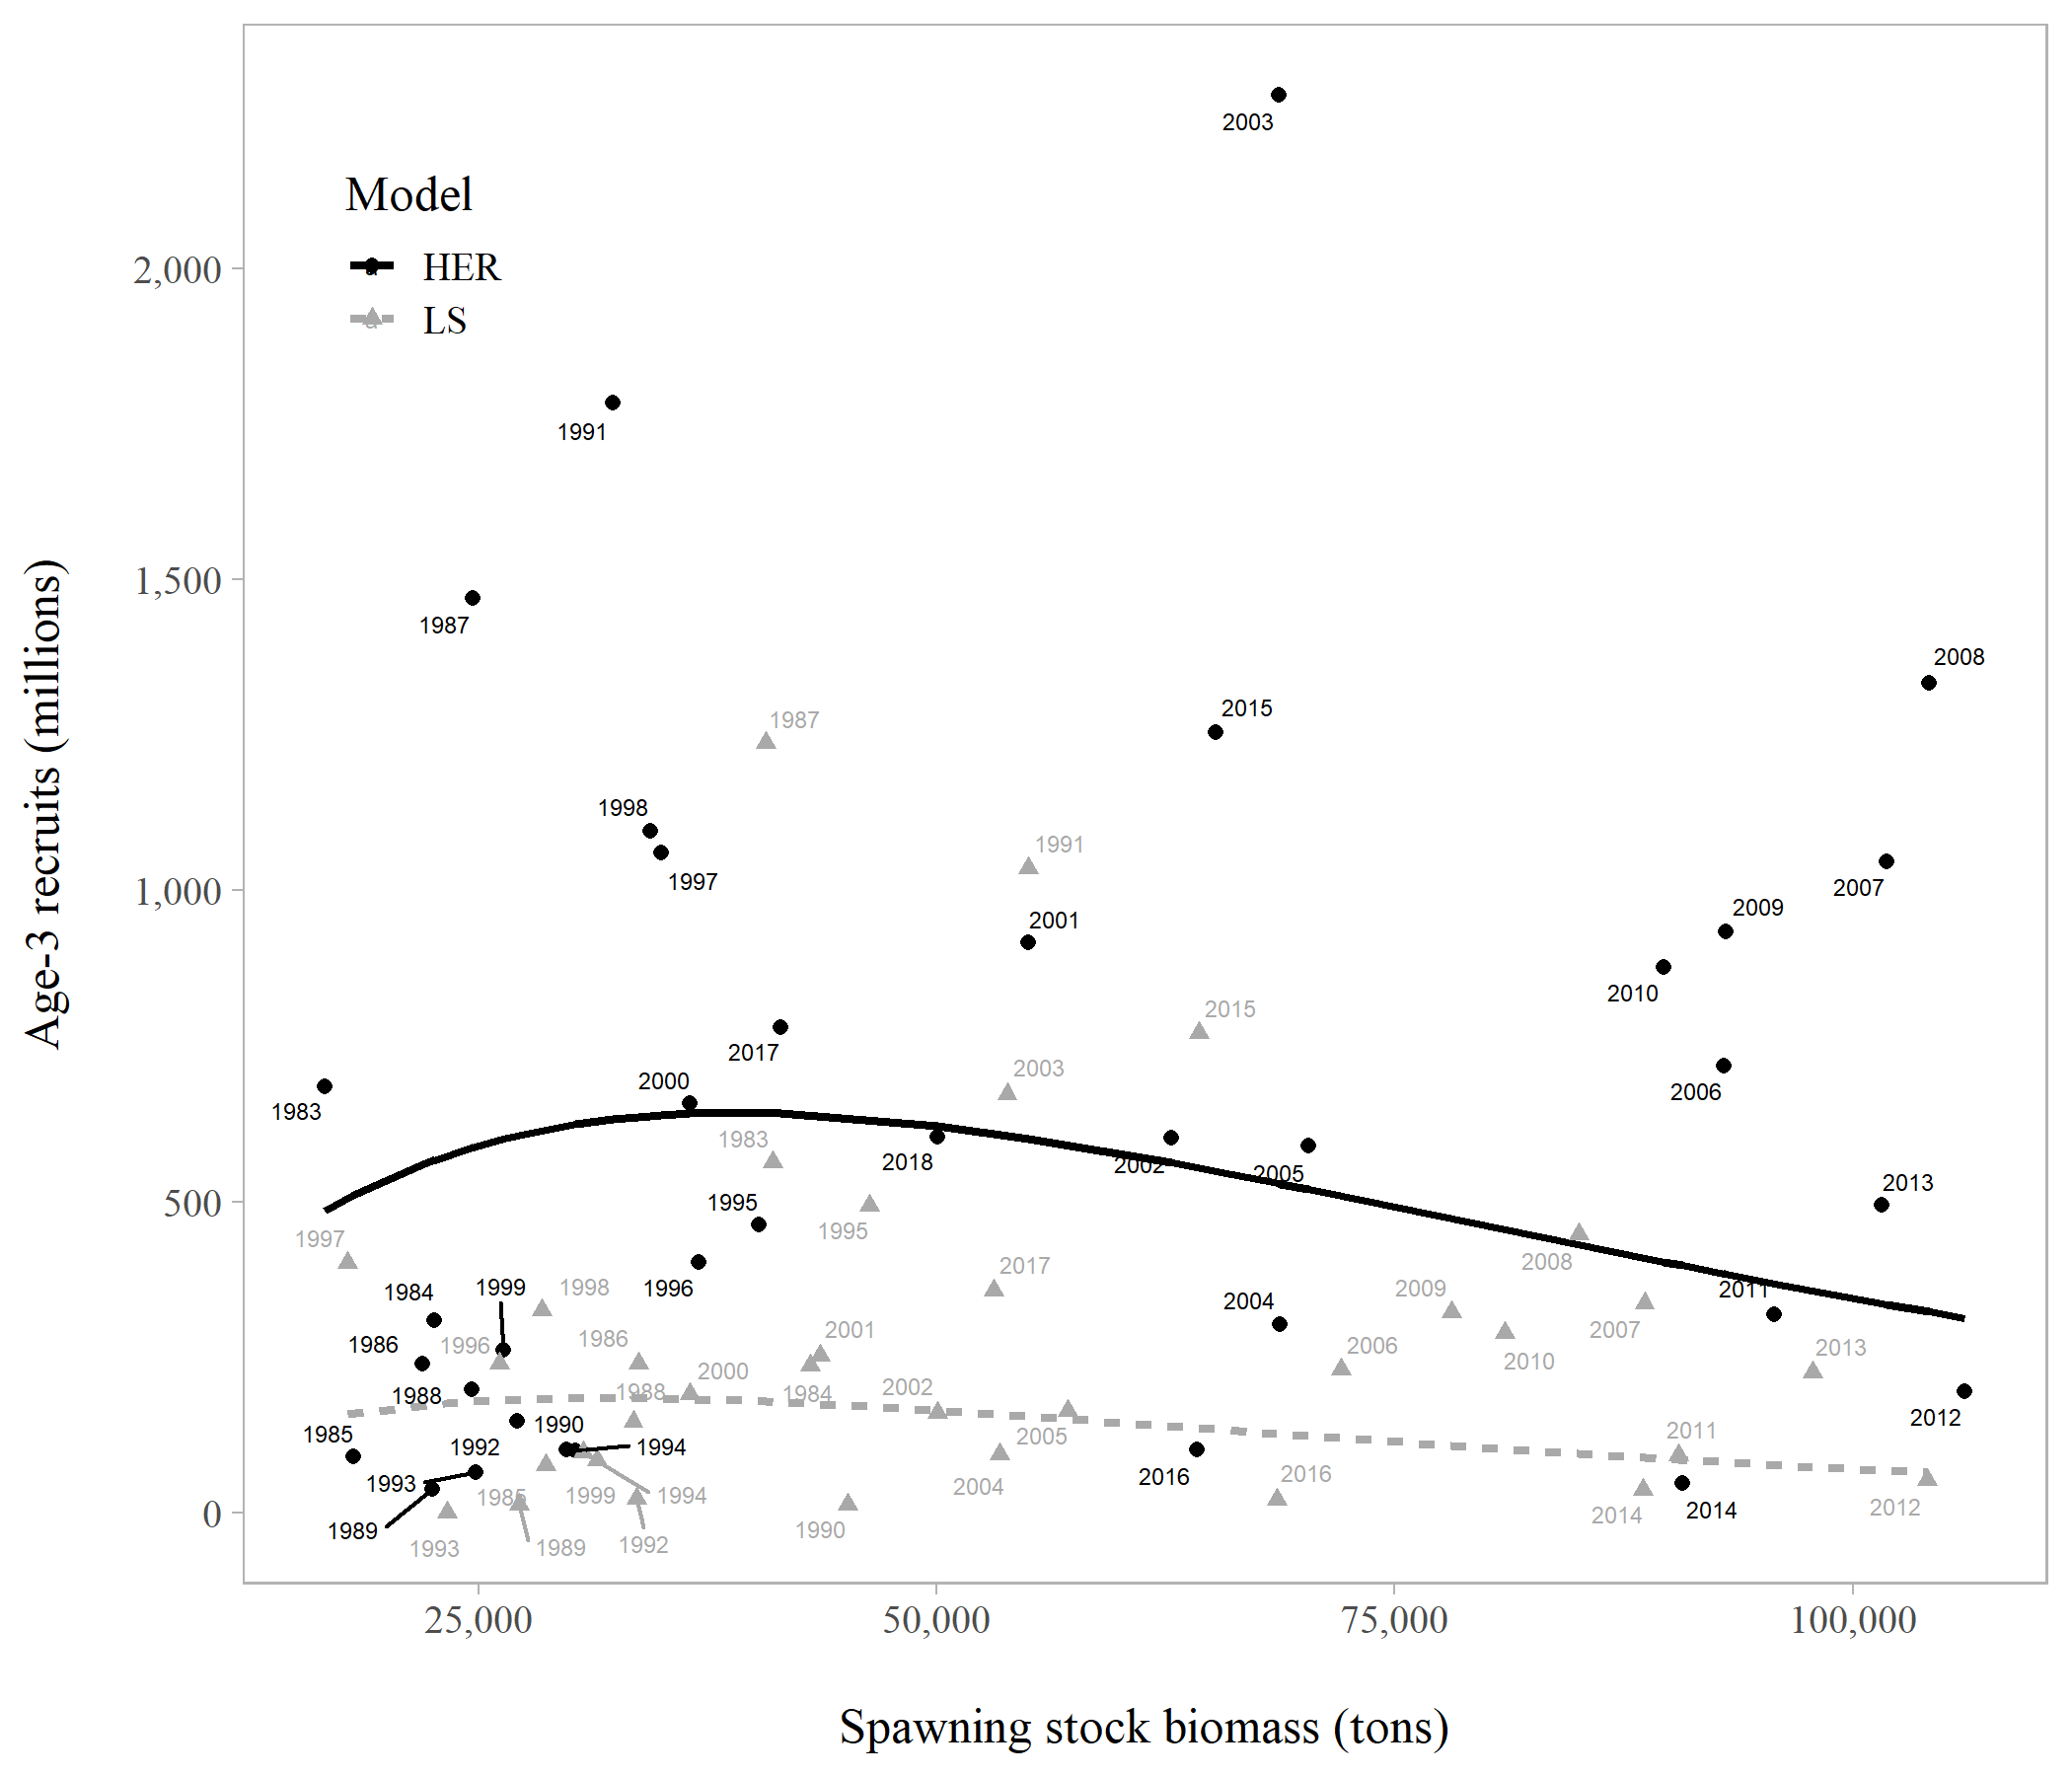
\includegraphics[width=1\linewidth]{../../HER/figs/compare_srcurves}

Figure 13. A comparison of annual estimates of age-3 recruits (millions)
versus spawning stock biomass (tons) in the age-structured model
(points) and Ricker model (lines) between HER (black circles and curve)
and LS (grey triangles and dashed curve).

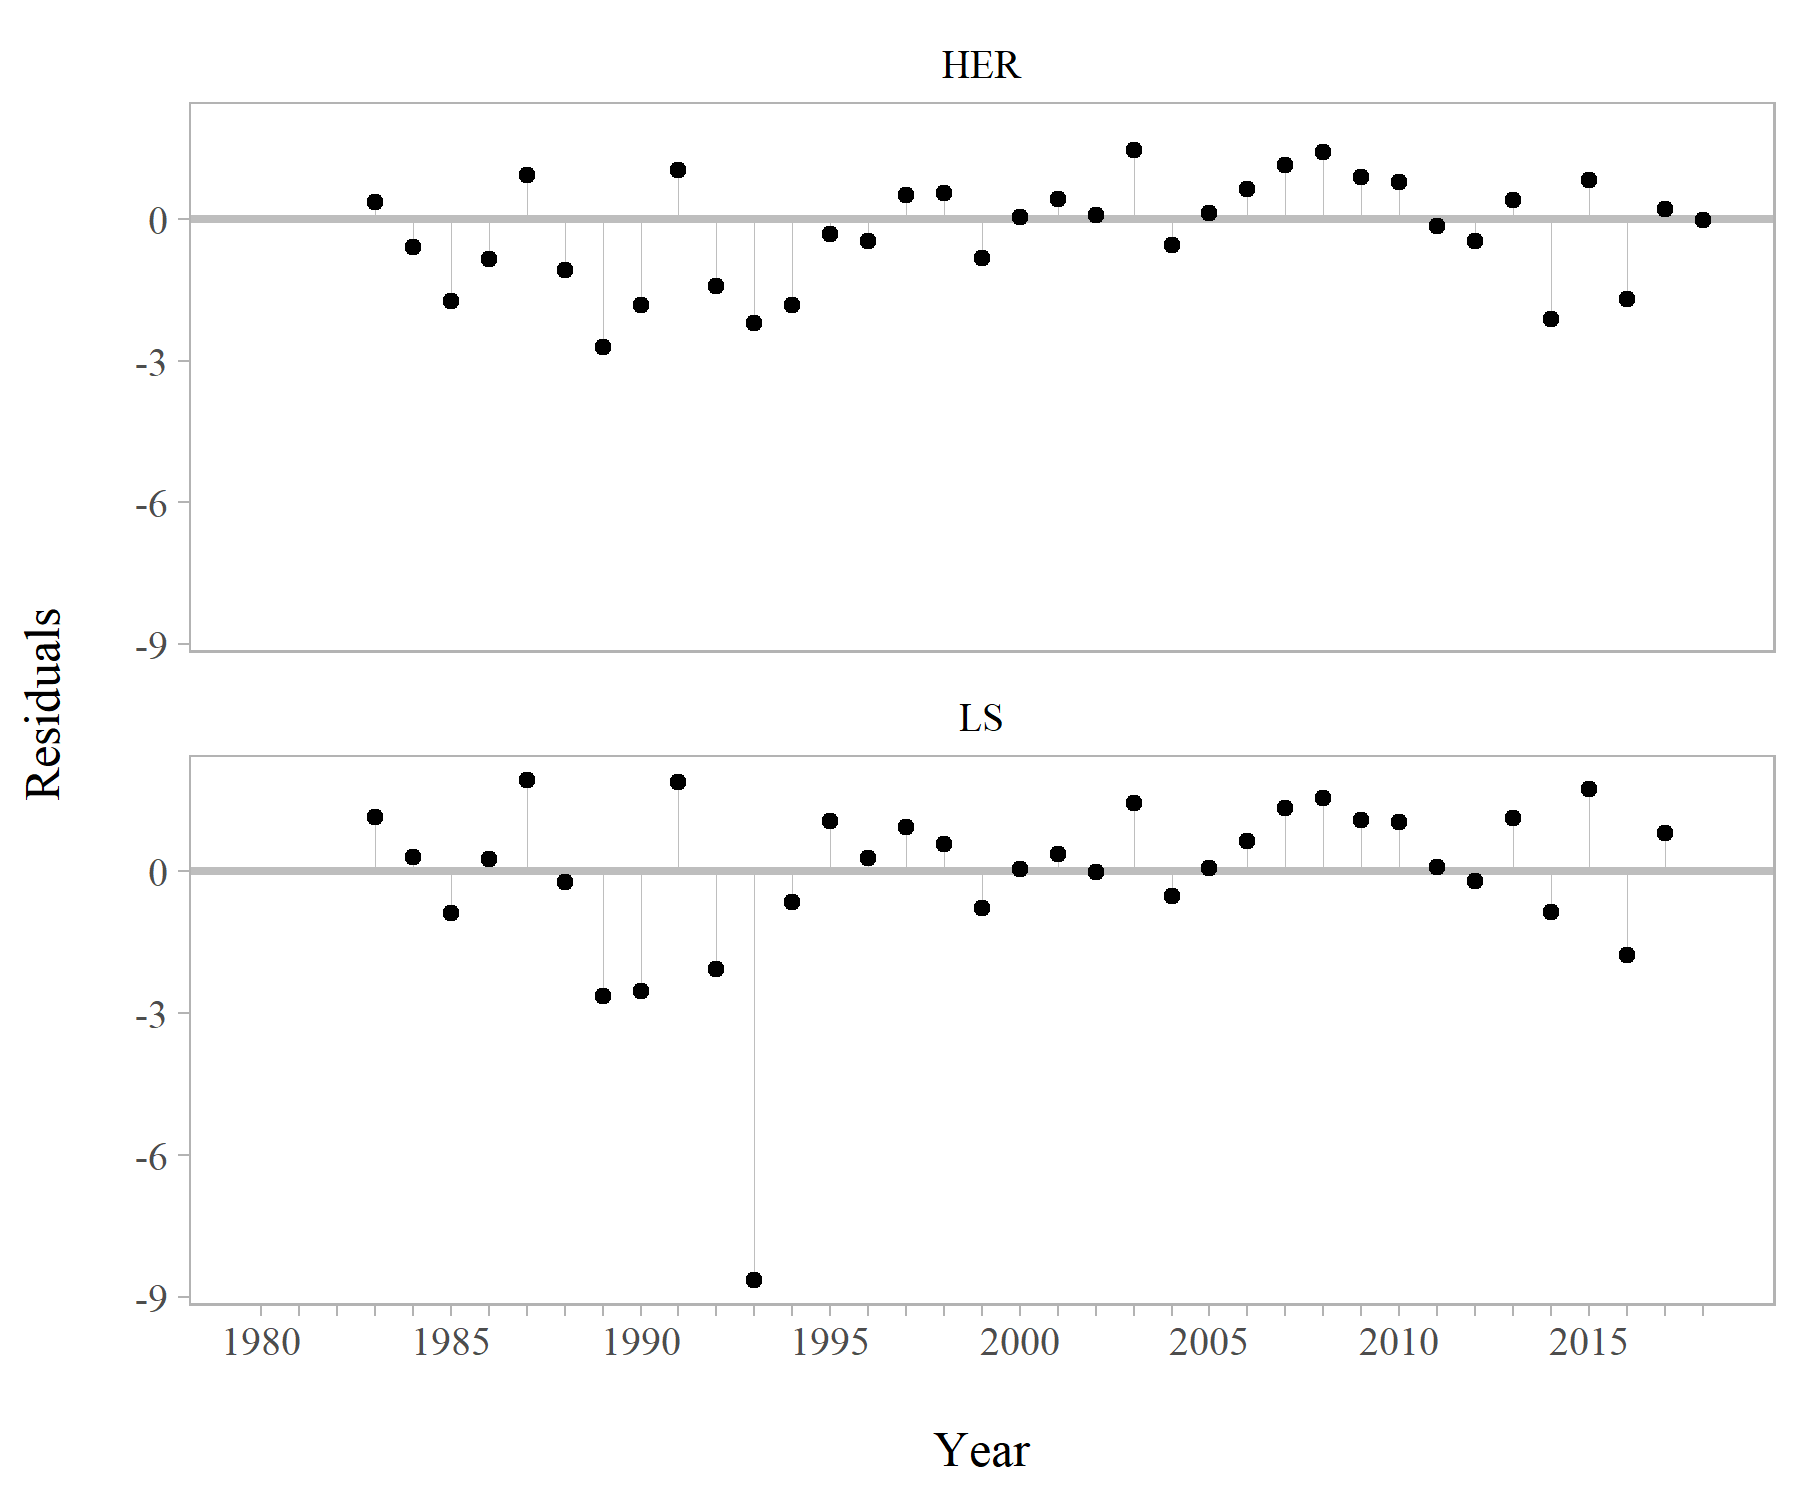
\includegraphics[width=1\linewidth]{../../HER/figs/compare_recruitresids}

Figure 14. A comparison of HER (top panel) and LS (bottom panel)
recruitment residuals calculated as the difference between age-3
recruits in the age-structured model and Ricker model on the logarithmic
scale.

\subsection{Next steps}\label{next-steps}

Sara would prefer the points in Figure 12 as side-by-side bars instead
of points, and to show the credibility interval around the ASA-estimated
points in Figure 13.

\section{Time-varying parameters}\label{time-varying-parameters}

Time varying parameters were quite different between LS and HER. Owing
to the way natural mortality \(M\) is estimating in HER (see \#1 under
section Differences between LS and HER), survival (-exp(\(M\))) appears
constant across time blocks in HER. Survival is very similar in HER and
LS between 1980 and 1998 (\textasciitilde{}0.57), but survival increases
dramatically in LS during the 1999-2014 time block corresponding to the
population increase during that period, and has dropped off slightly
since 2015 (Figure 15). The inability for the HER model to vary \(M\)
likely contributes to the model's poor fit and residual patterns in
mature biomass (Figure 1), egg deposition (Figure 6), and age
compositions (Figure 8).

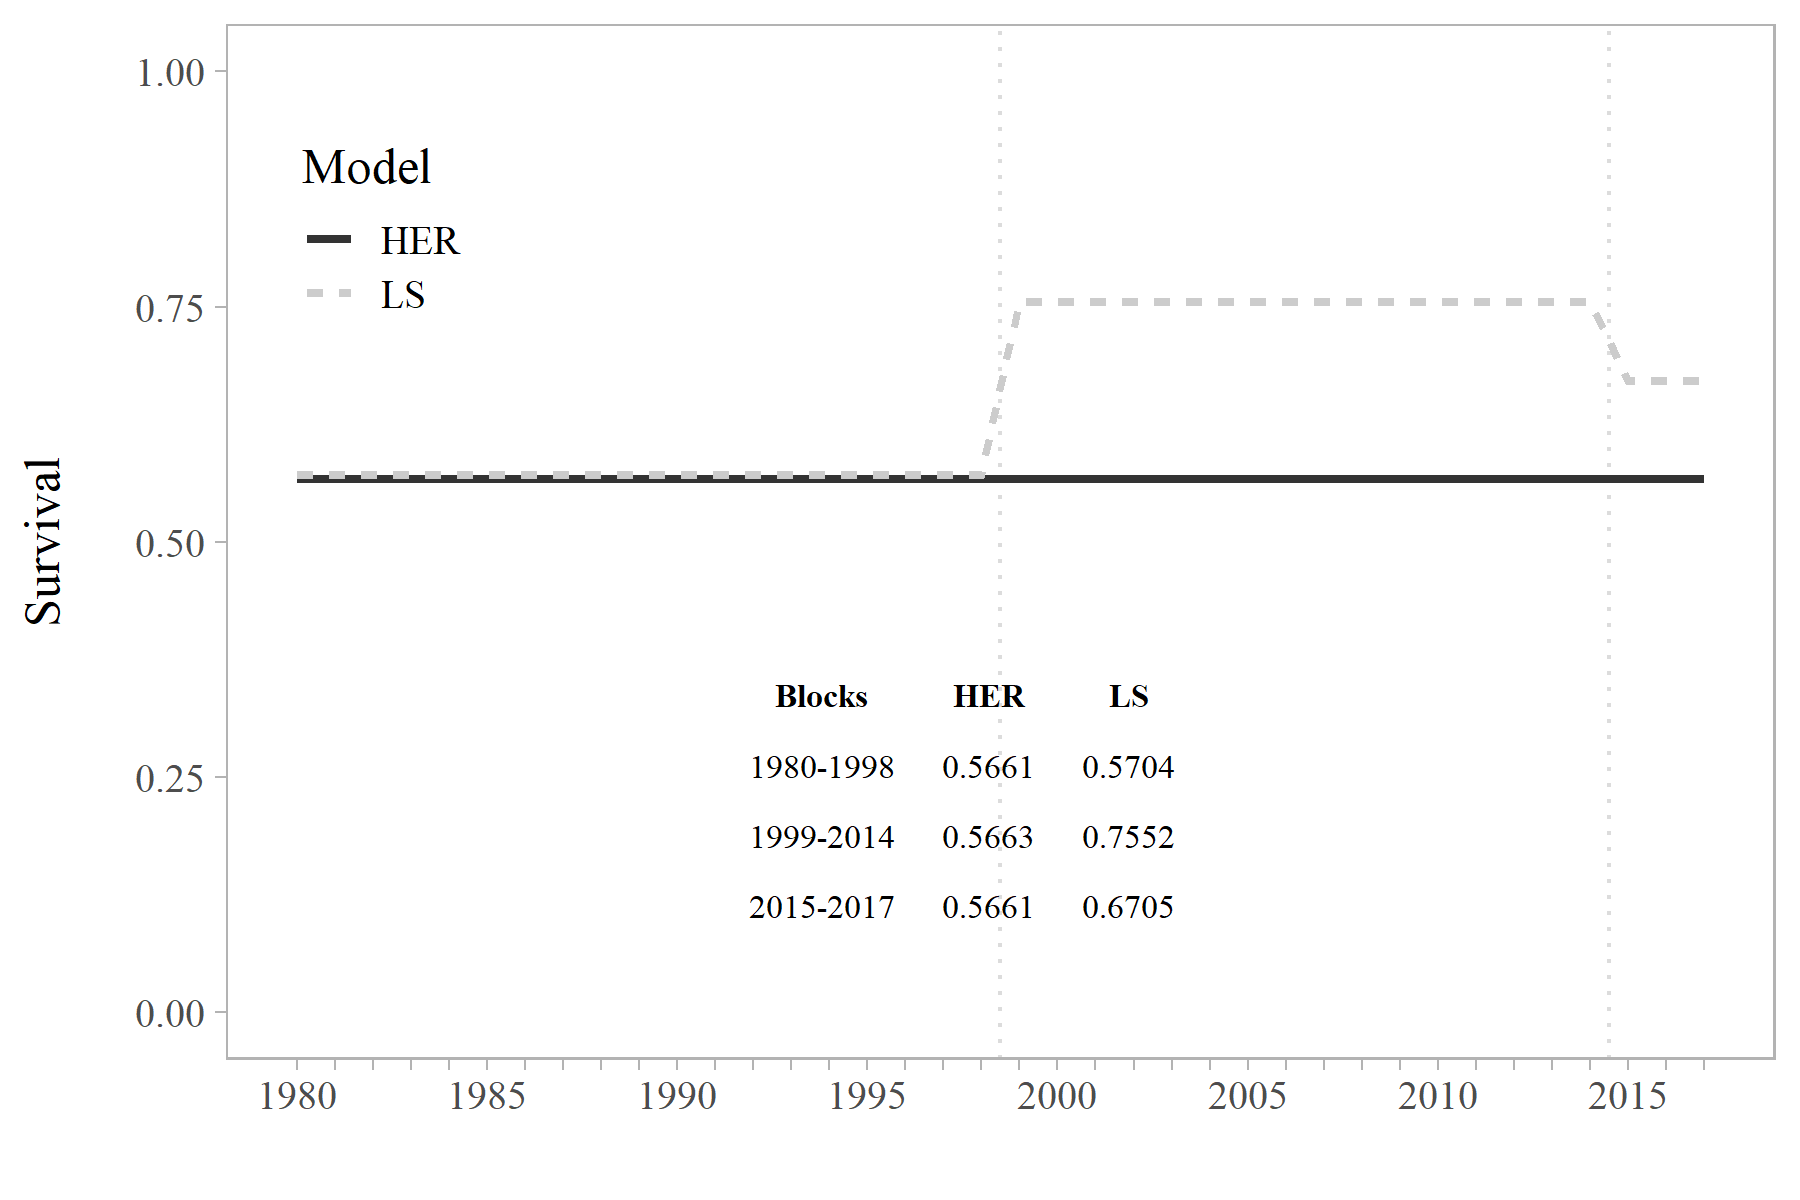
\includegraphics[width=1\linewidth]{../../HER/figs/compare_survival}

Figure 15. A comparison of HER (black solid line) and LS (grey dashed
line) model estimates of survival by time block.

The LS model estimates of matuirty-at-age in both time block suggest
herring mature at a much younger age than what is predicted in HER
(Figure 16). Similarly, the LS model predicts that a greater
proportion-at-age selects to the gear than HER (Figure 16). In HER,
selectivity was scaled to have a mean of 1 across all ages in log space
by substracting the mean from the vector of age-specific selectivities.
We normalized it betweeb 0 and 1 in order to directly compare the
estimated selectivity-at-age between HER and LS by dividing
selectivity-at-age by the maximum selectivity.

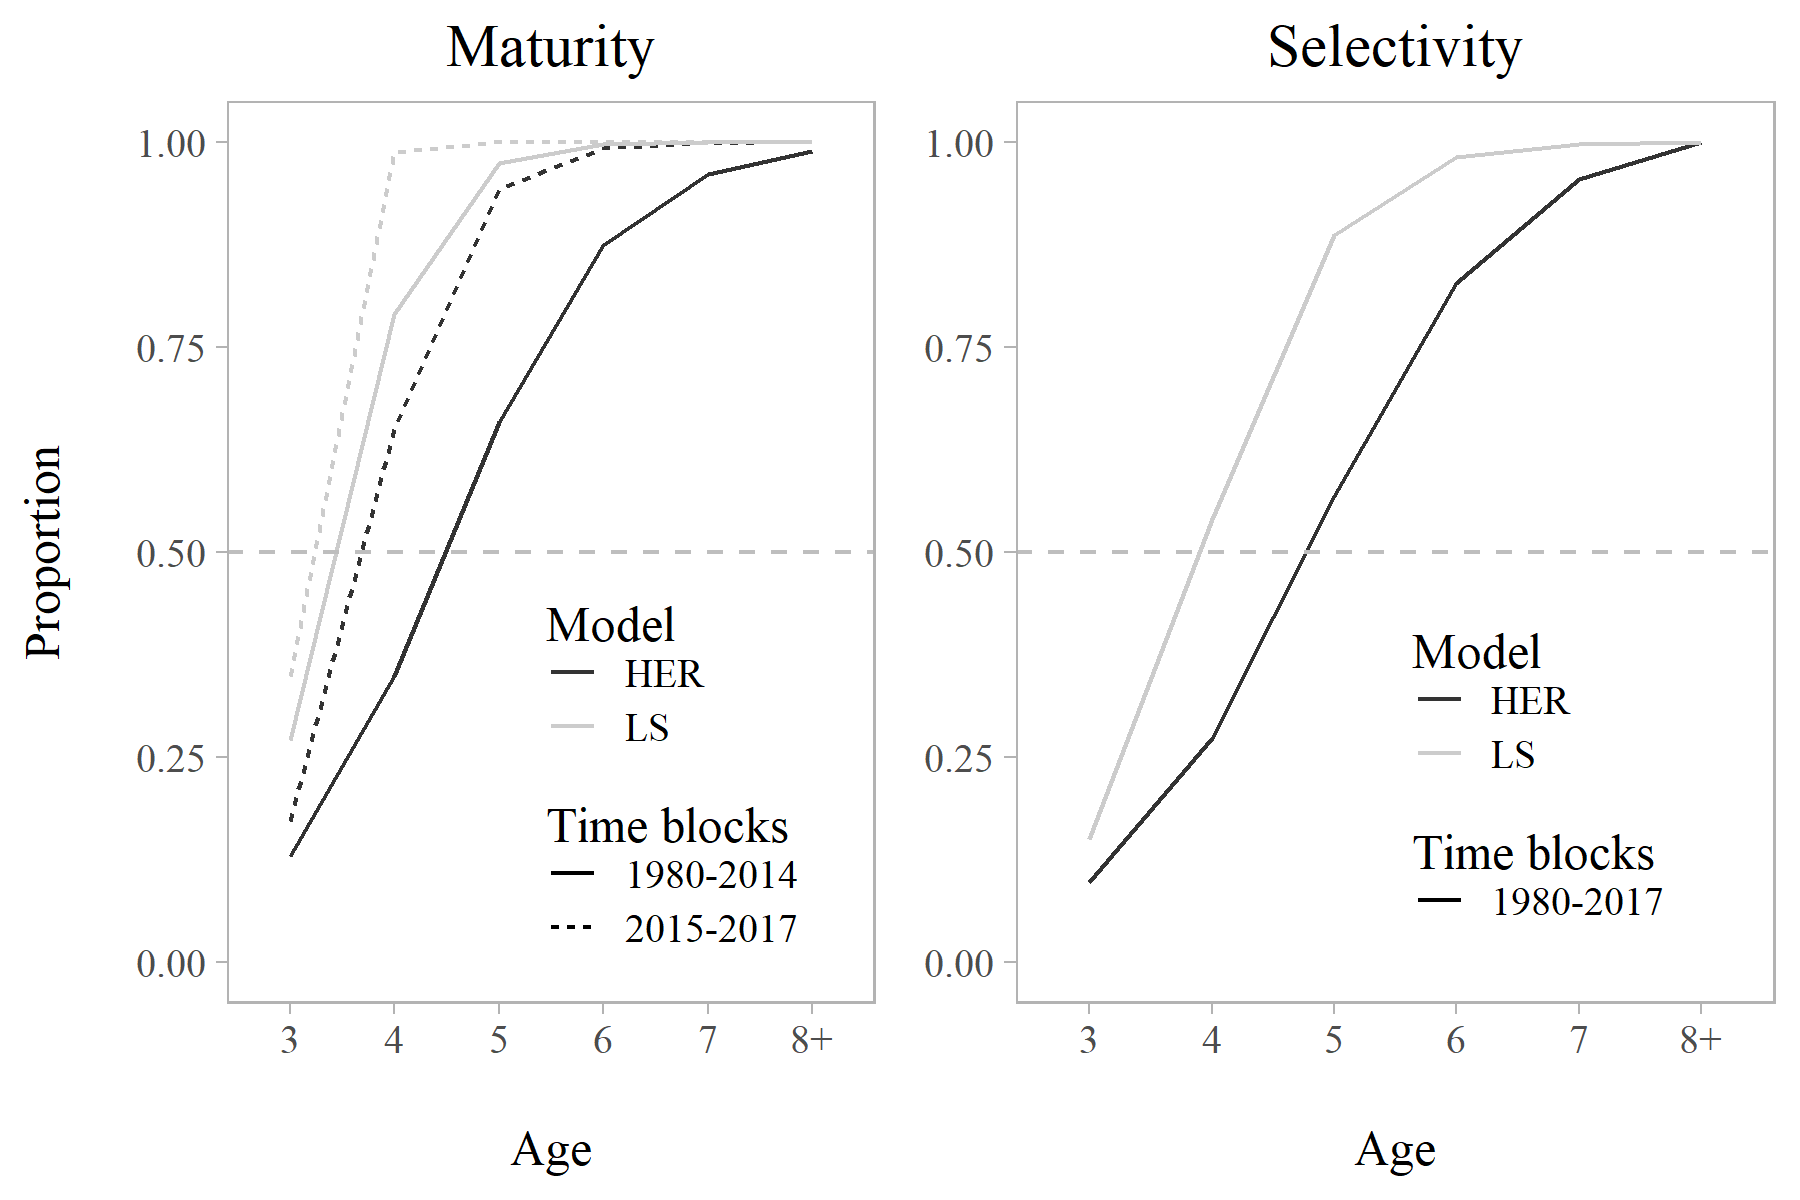
\includegraphics[width=1\linewidth]{../../HER/figs/compare_mat_sel}

Figure 16. A comparison of HER (black) and LS (grey) model estimates of
maturity (left panel) and selectivity (right panel) by time block.

\section{Weight-at-age}\label{weight-at-age}

Fish and Game uses weight-at-age from the fishery for both fishery and
spawner weight-at-age in both LS and HER, because there are too many
spawned out fish collected in cast net that may bias samples. The only
exception is 1997, when cast net samples were used for spawner
weight-at-age because the weight-at-age in the fishery was deemed to be
too high.

Weight-at-age has been quite variable in the Sitka herring stock, as
evidenced by cohort-specific trends (Figure 17) and trends by sampling
year (Figure 18).

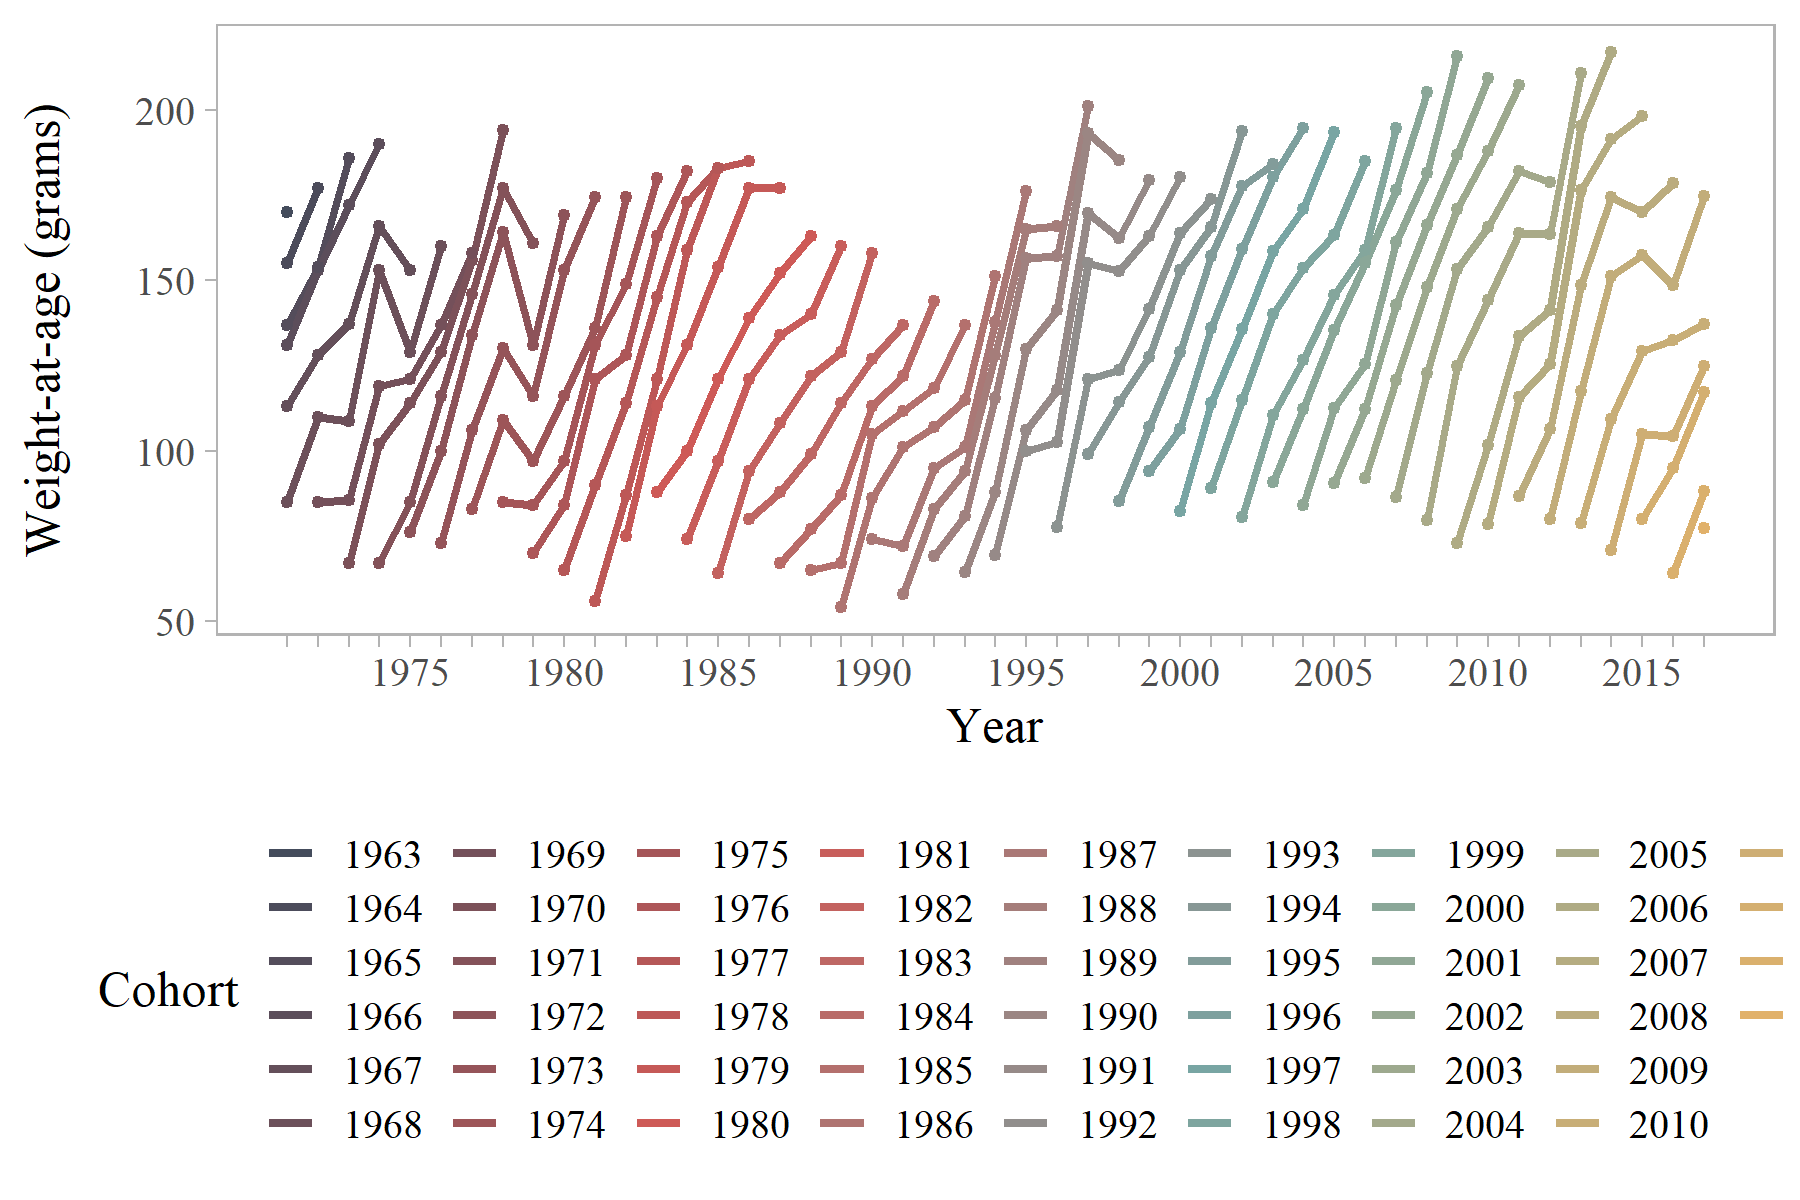
\includegraphics[width=1\linewidth]{../../HER/figs/waa_cohort_plot}

Figure 17. Commercial catch weight-at-age (grams) by cohort.

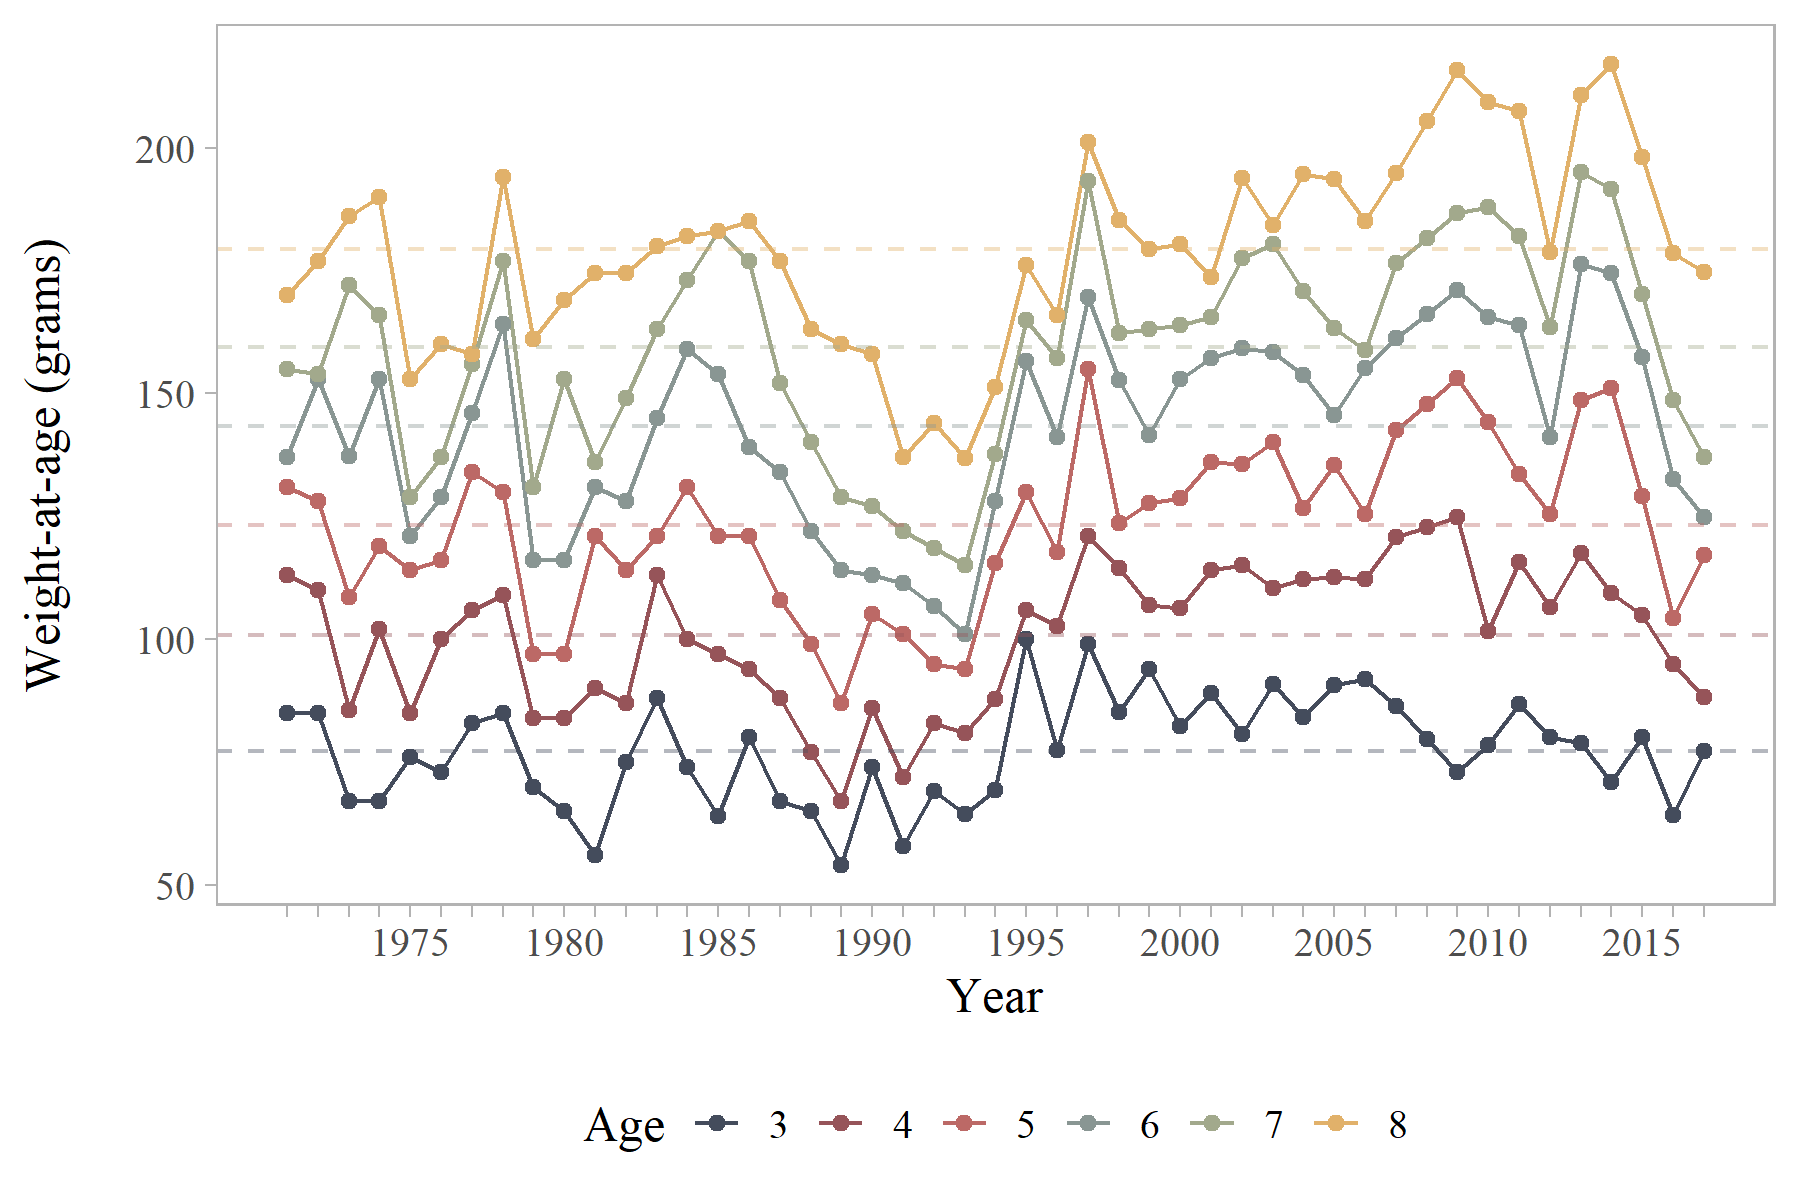
\includegraphics[width=1\linewidth]{../../HER/figs/waa_plot}

Figure 18. Weight-at-age (grams) by sampling year. Mean weight by age
class over time is shown in the dashed lines.

\subsection{Next steps}\label{next-steps-1}

Remove age-8 from these figures because it's the plus group.

\section{Variance estimate using
MCMC}\label{variance-estimate-using-mcmc}

Estimating variance in ADMB can be split into a series of smaller
objectives: 1) determining quantities of interest, 2) generating output
files for posterior samples on quantities, 3) writing R code for
implementing MCMC in ADMB, including determining number of iterations
and proper thinning, and 4) writing R code for testing convergence
diagnostics, variance estimation, and visualization of results.

With the help of Sherri and Sara, we determined quantities of interest
for variance to be: - Mature biomass (pre-fishery) - Spawning stock
biomass (post-fishery) - Forecast mature biomass - Natural
mortality/survival - Recruitment \emph{Needs to be updated, see Next
steps} - Maturity - Selectivity - Catch (I added this, but it only works
when conditioning on effort - conditioning on catch assumes zero
variance) - Egg deposition

The HER.tpl file now contains code to sample the posterior distributions
for all of these quantities. One roadblock to this was the fact that the
population dynamics model for HER had several differences that made it
challenging to derive specific quantities of interest. These have by and
large been corrected, and this is no longer an issue. The notable
exception is that the assumptions about catch being mature are different
in the least-squares (LS) and HER models. I've been in contact with S.
Dressel and S. Miller about this via email since 2018-07-30.

The her.R script contains a few functions to tidy and visualize output
from the posterior samples of quantities of interest. I also wrote
sample/example code to visual confidence intervals (e.g.~Figure 19),
examine diagnostic caterpillar plots for both derived quantities
(e.g.~Figure 20) and age-based or time-varying quantities (e.g.~Figure
21), and look at the posterior densities (e.g.~Figure 22 and Figure 23).
As indicated by the diagnostic caterpillar plots, the MCMC chain was not
run for long enough to ensure convergence or full mixing.

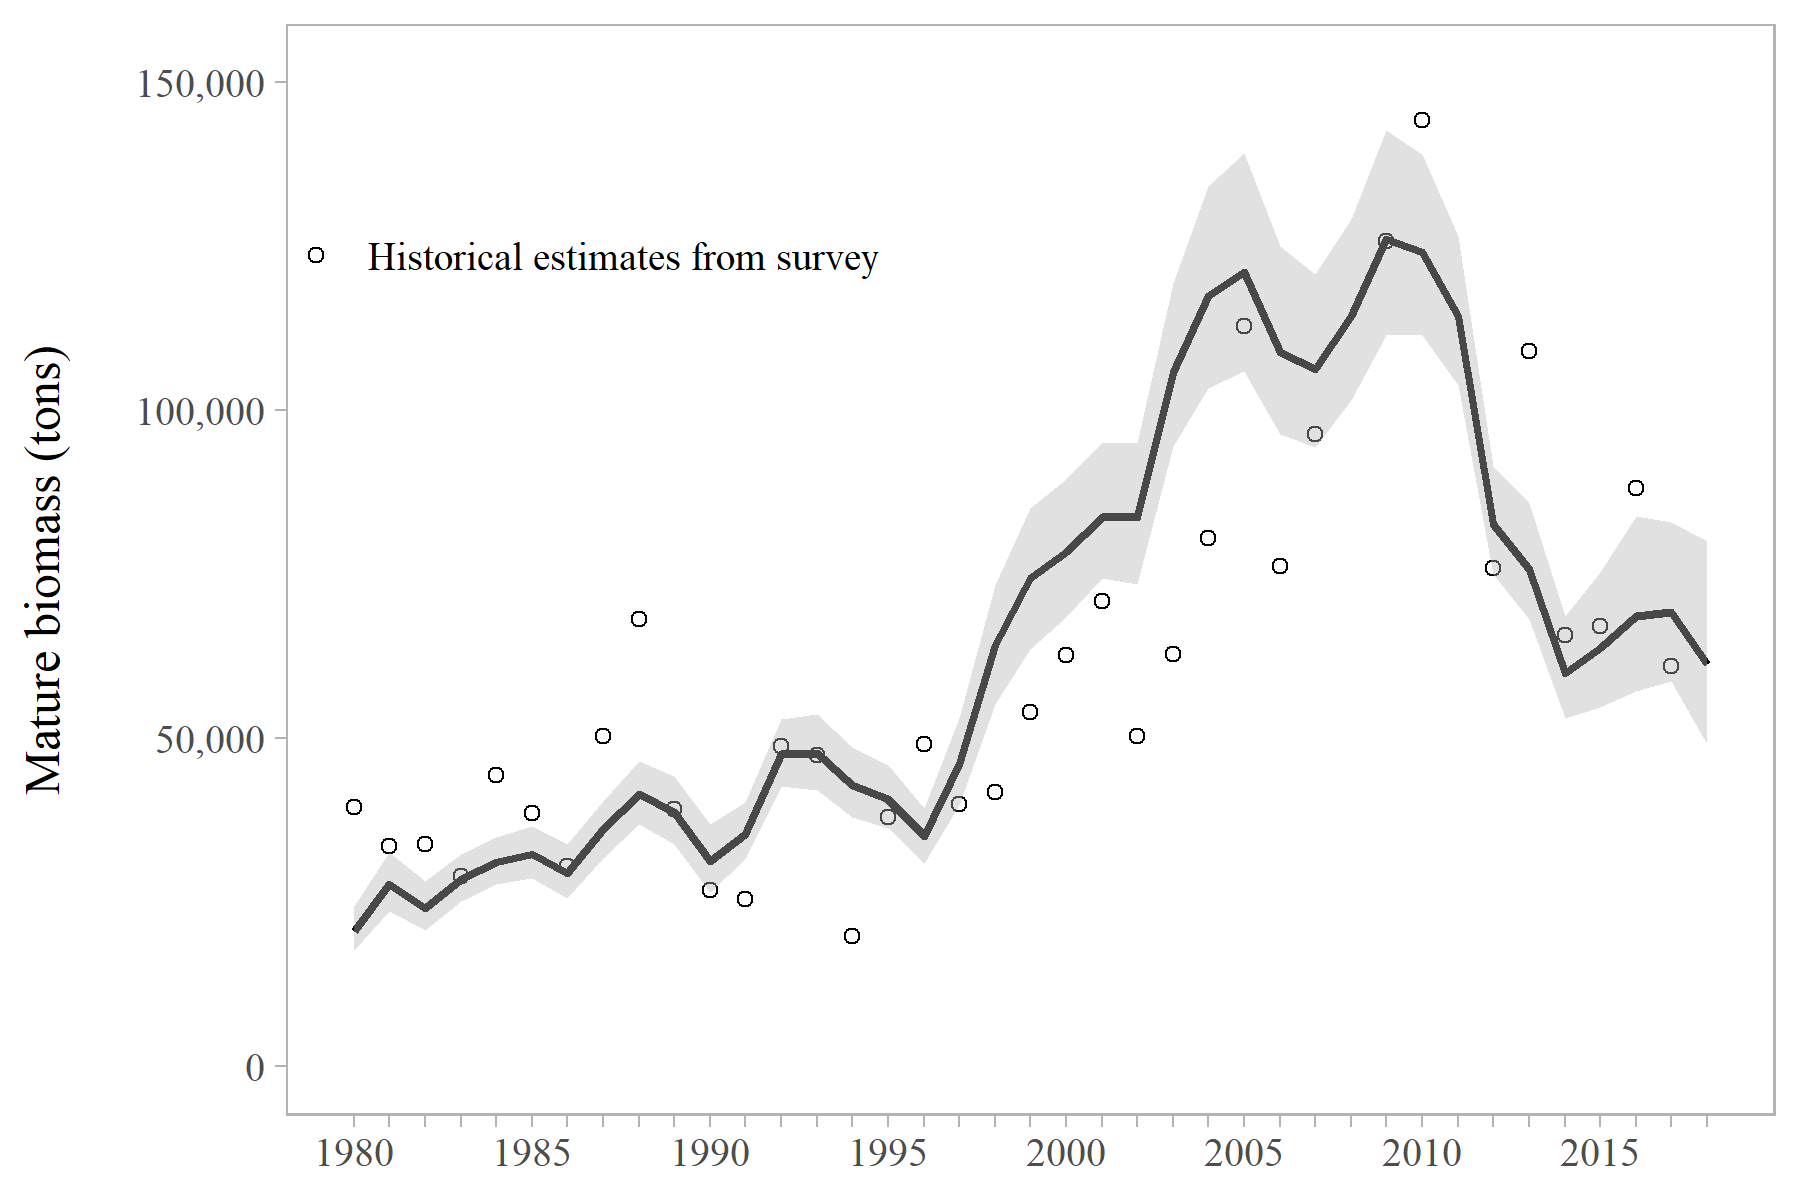
\includegraphics[width=1\linewidth]{../../HER/figs/HER/matbiomass_mcmc_plot}

Figure 19. An example of visualizing the 95\% credibility intervals for
mature biomass.

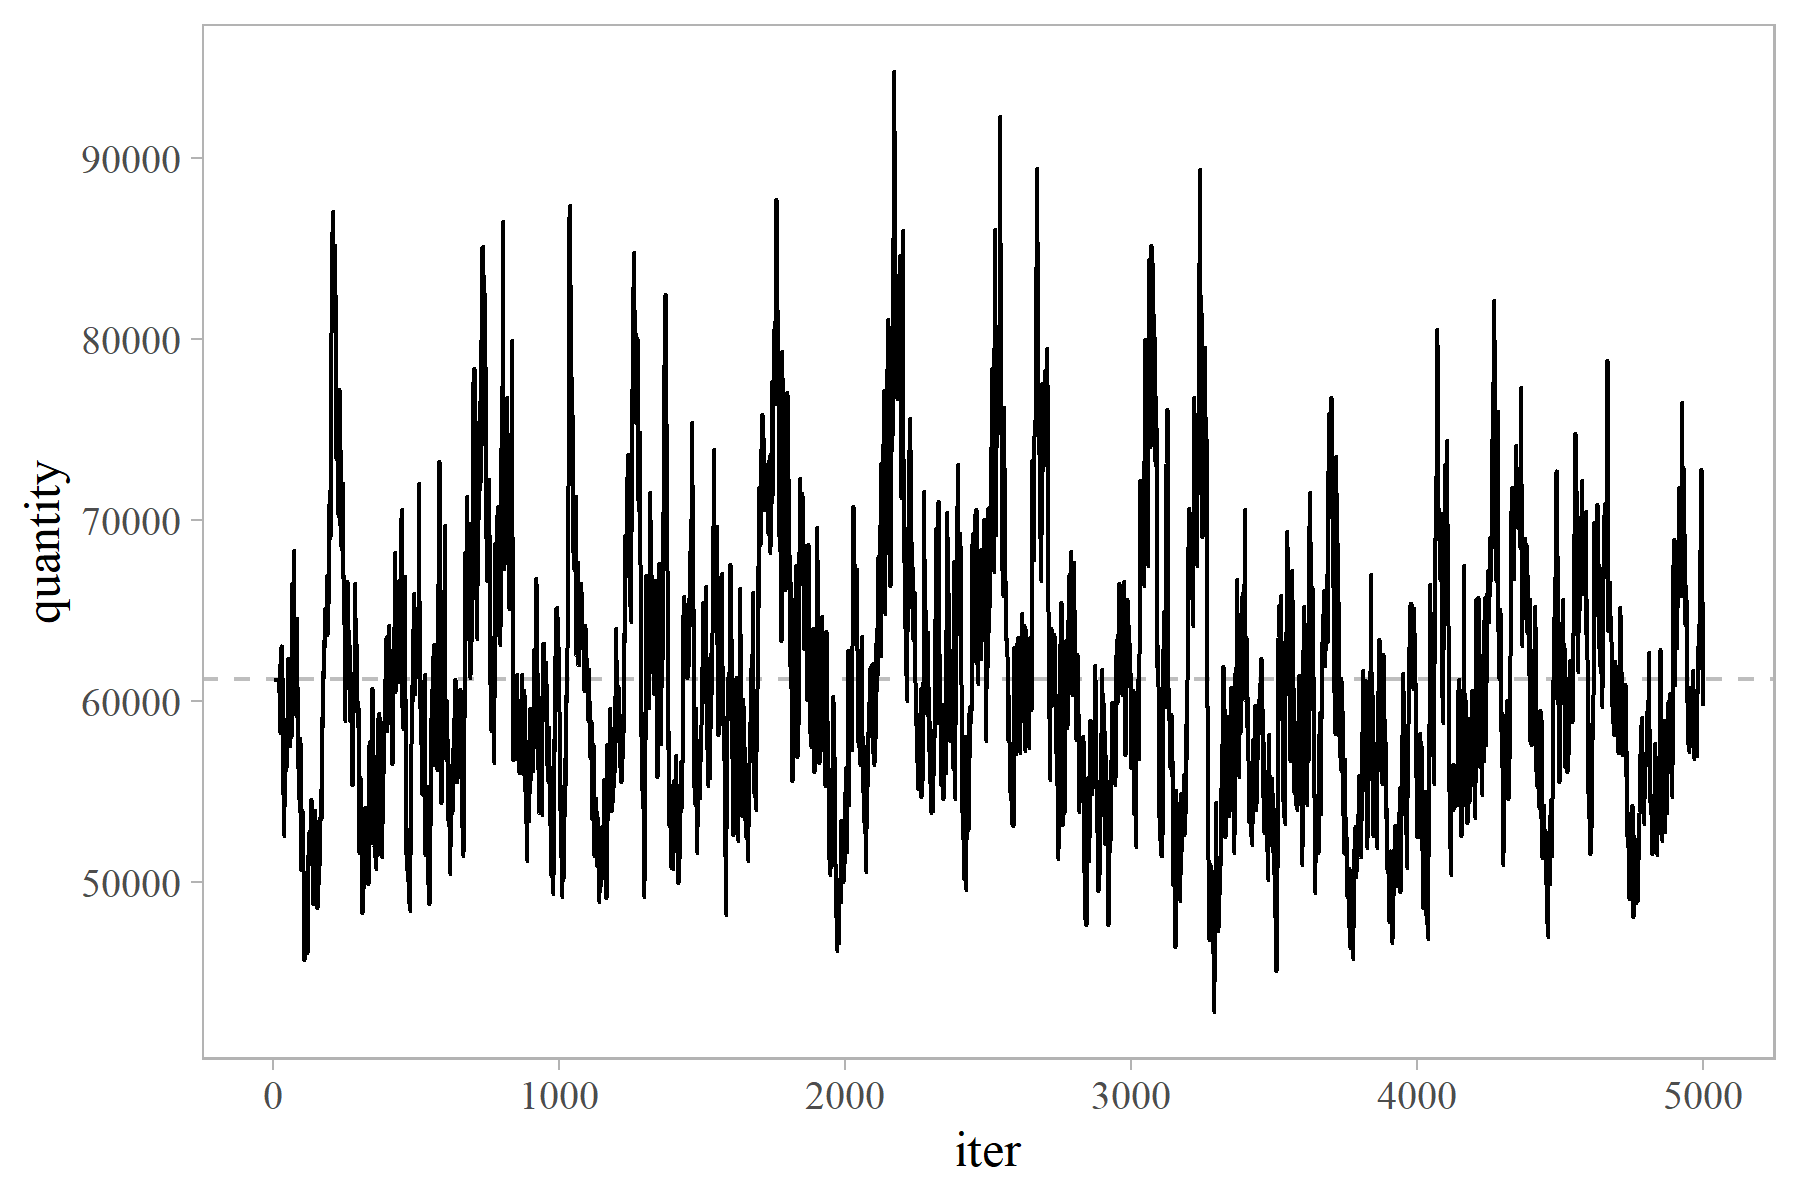
\includegraphics[width=1\linewidth]{../../HER/figs/HER/caterpillar_forematb}

Figure 20. An example of a diagnostic caterpillar plot for forecasted
mature biomass.

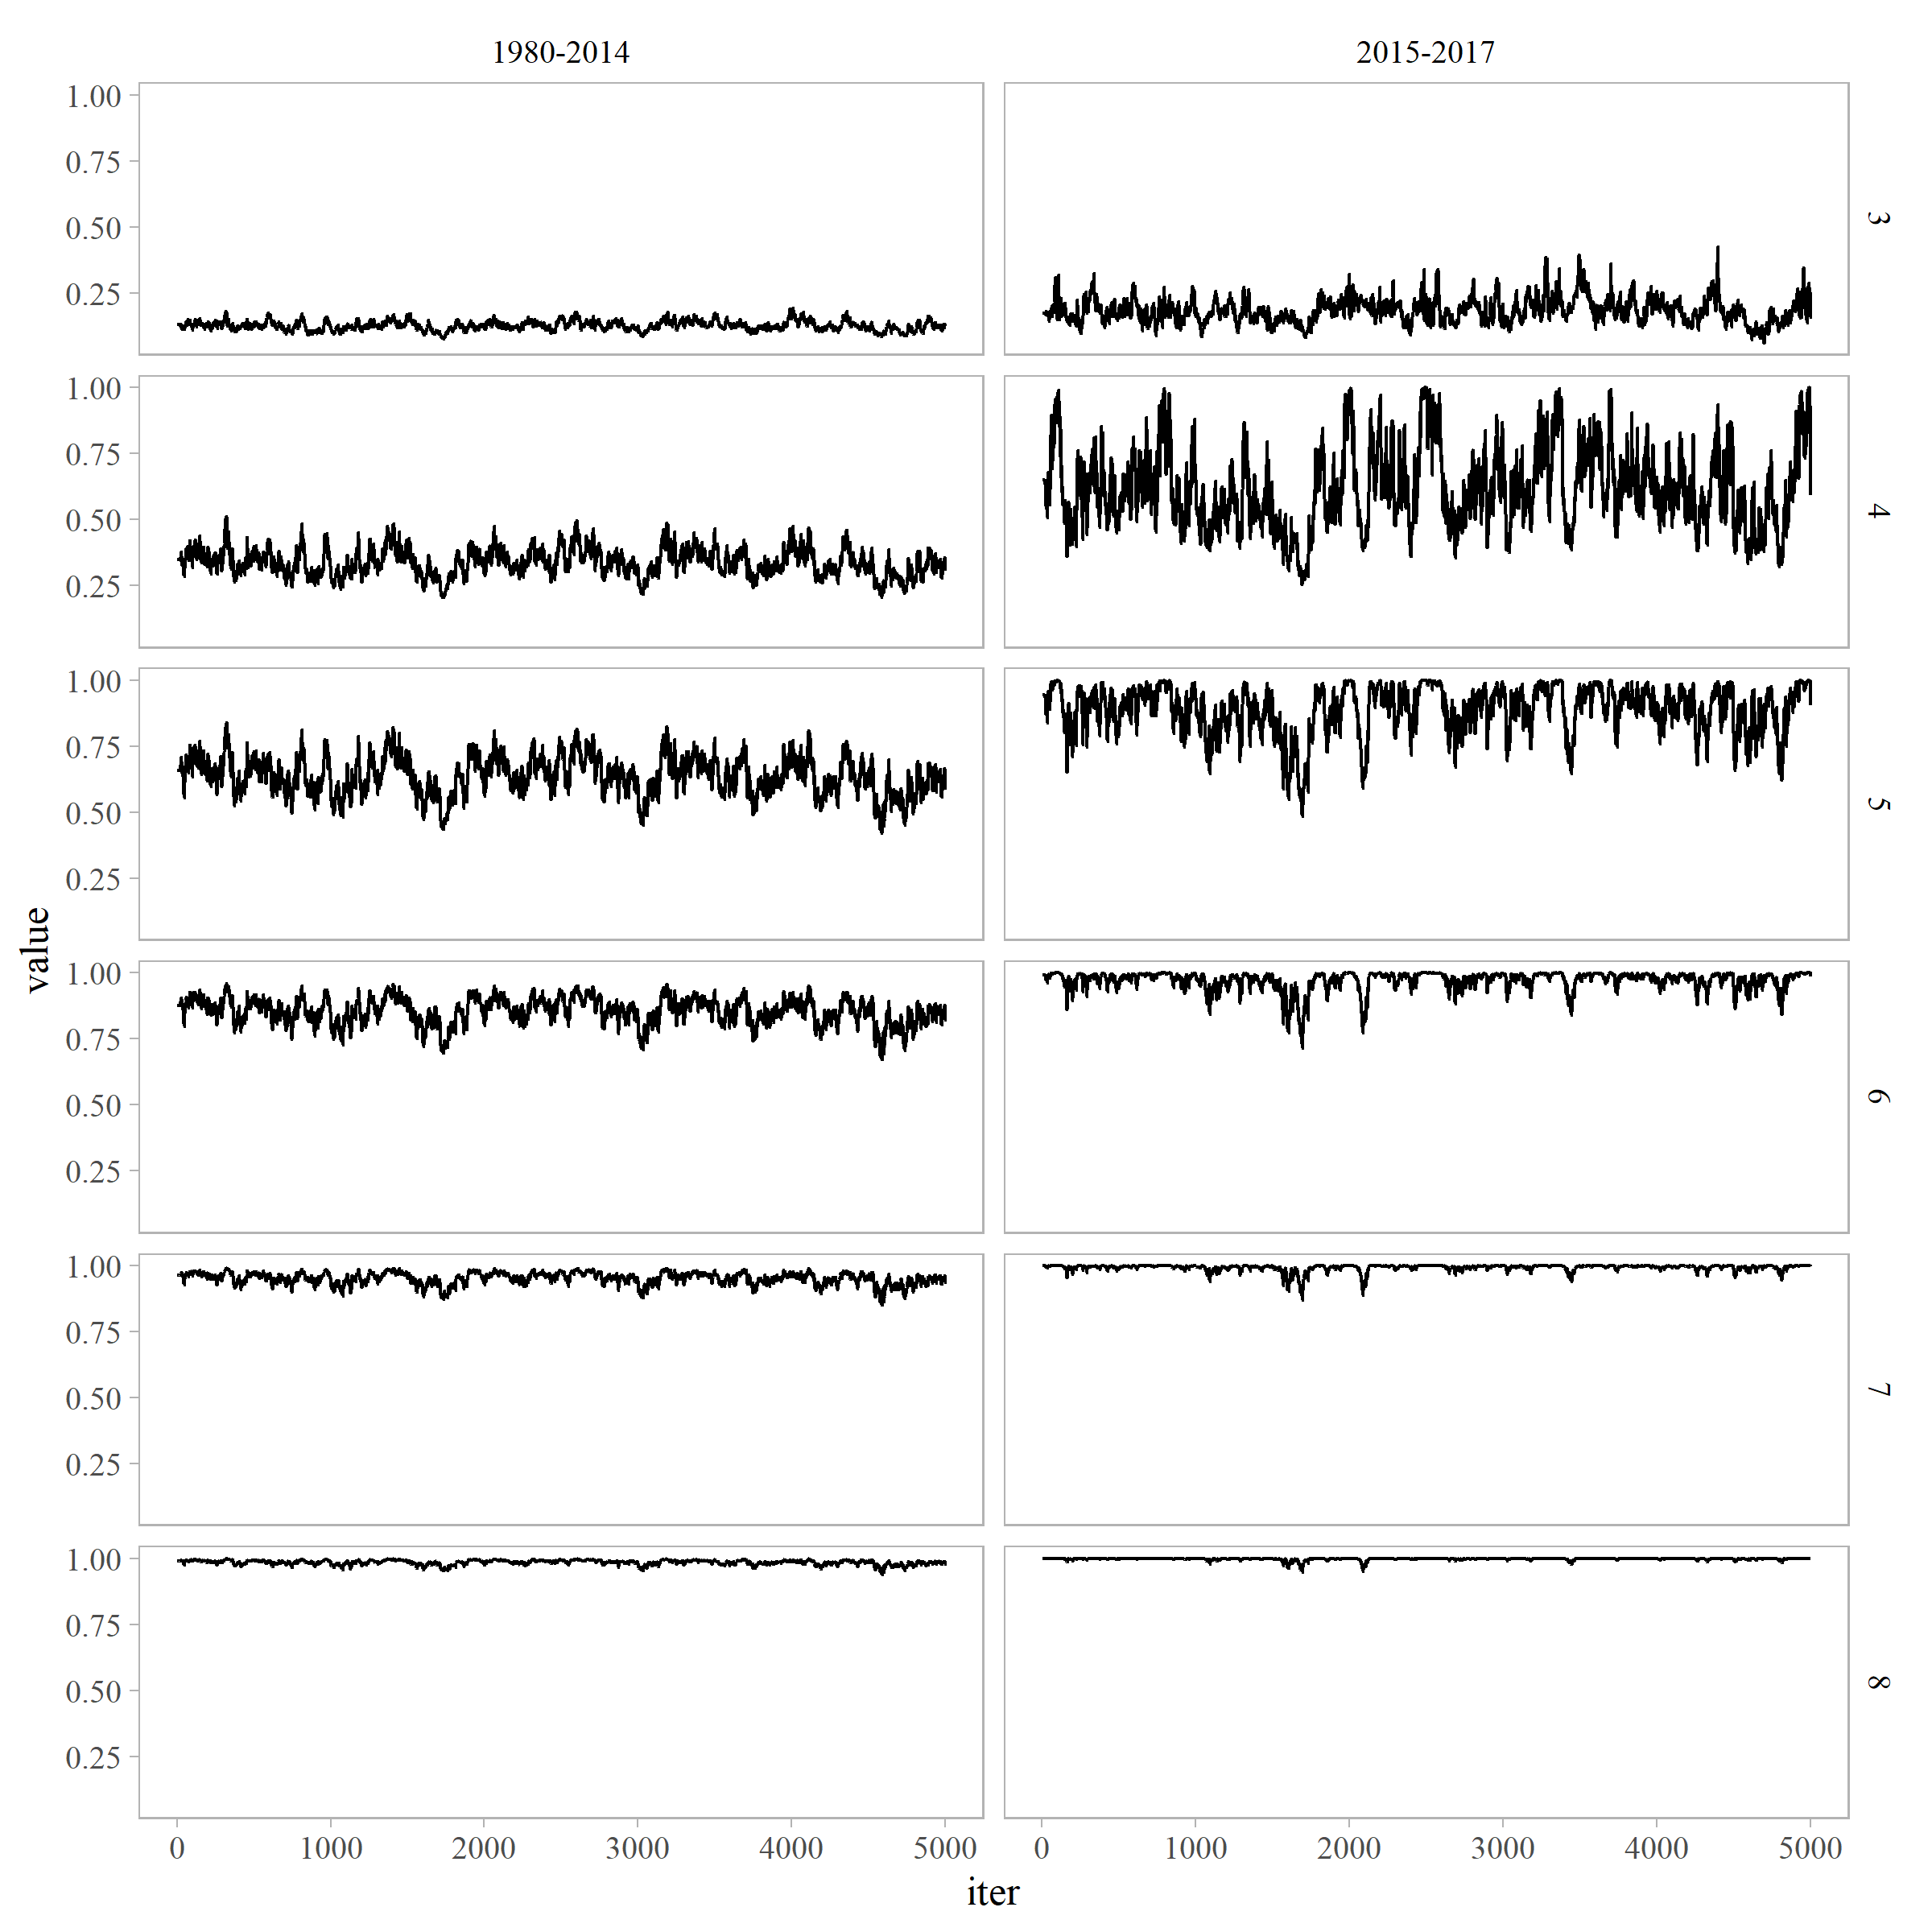
\includegraphics[width=1\linewidth]{../../HER/figs/HER/caterpillar_mat}

Figure 21. An example of a diagnostic caterpillar plot for an
age-structure and time-varying parameter.

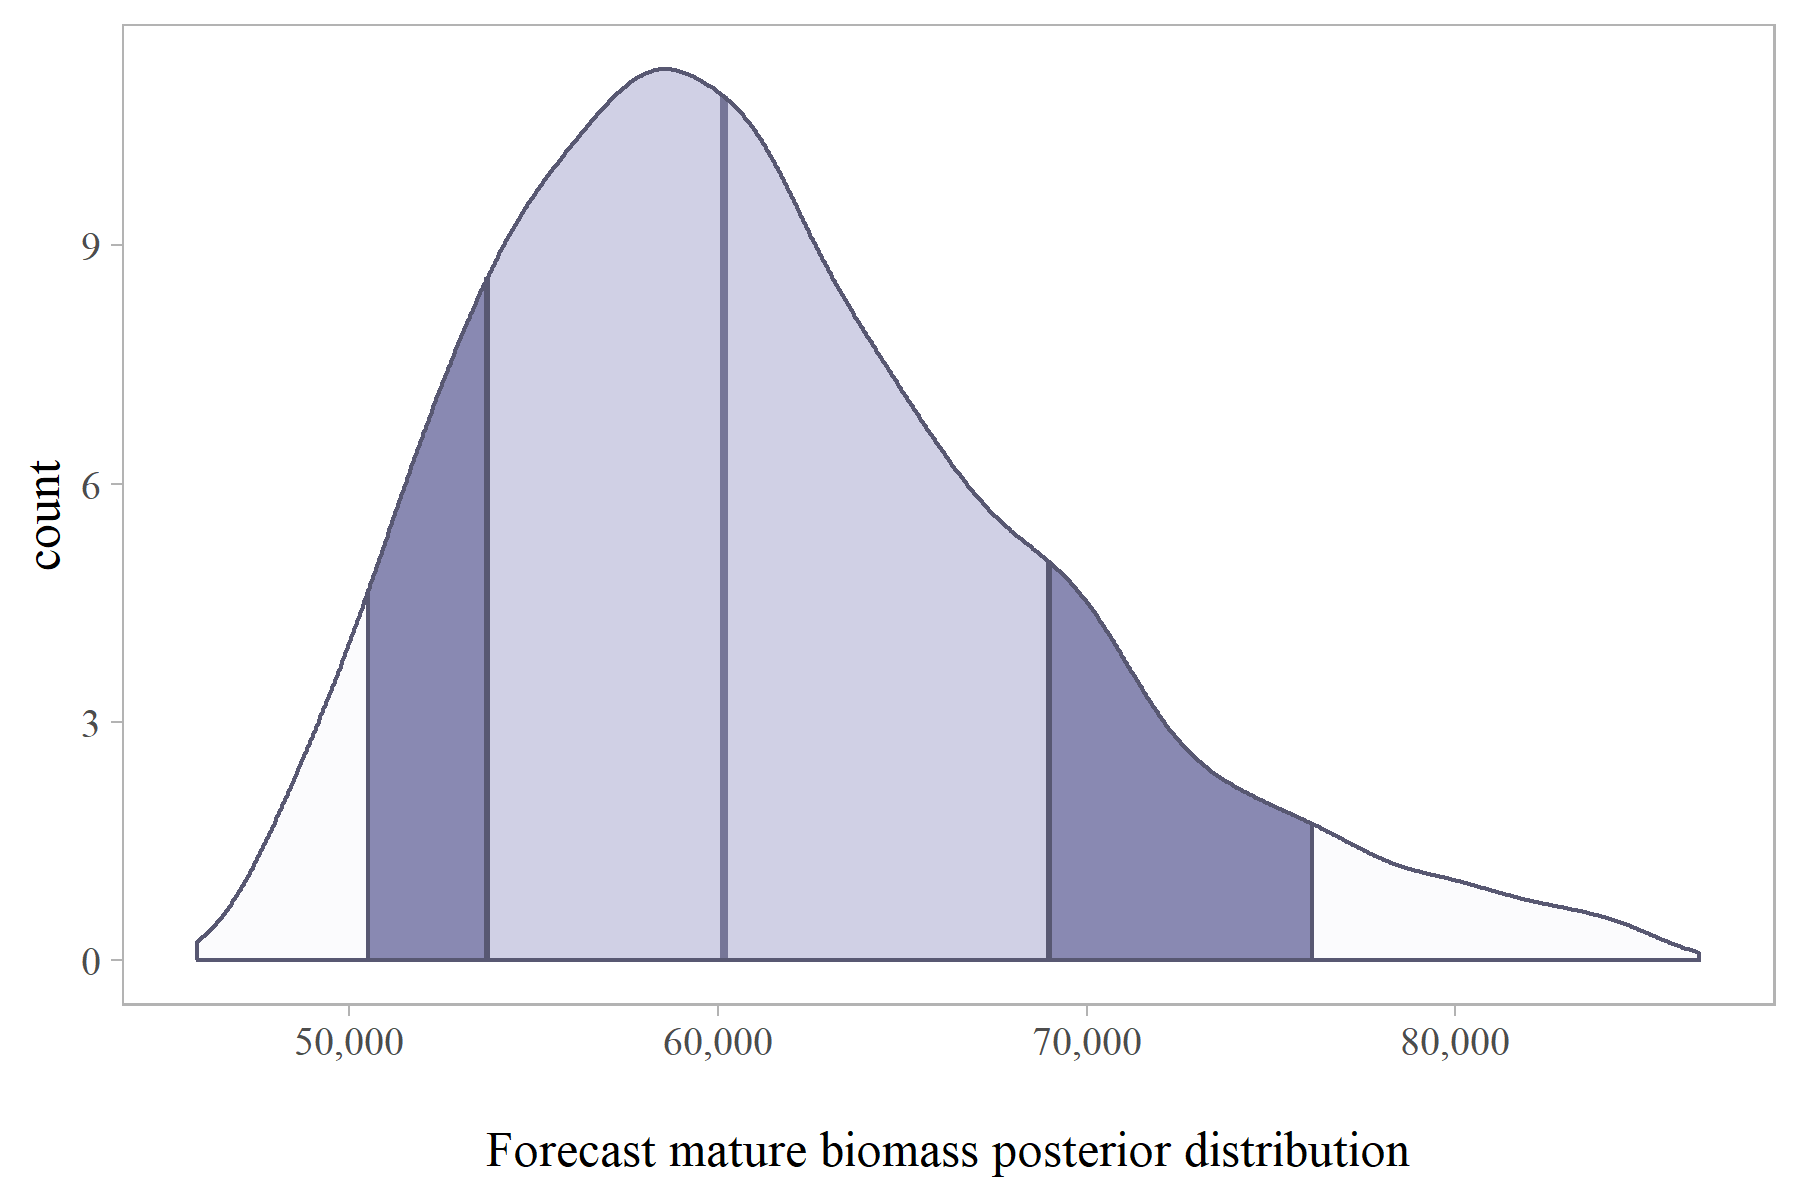
\includegraphics[width=1\linewidth]{../../HER/figs/HER/posterior_forematb}

Figure 22. The full posterior densities of mature biomass, including the
median (line) and 50\% (lighter shading) and 95\% percentiles (darker
shading).

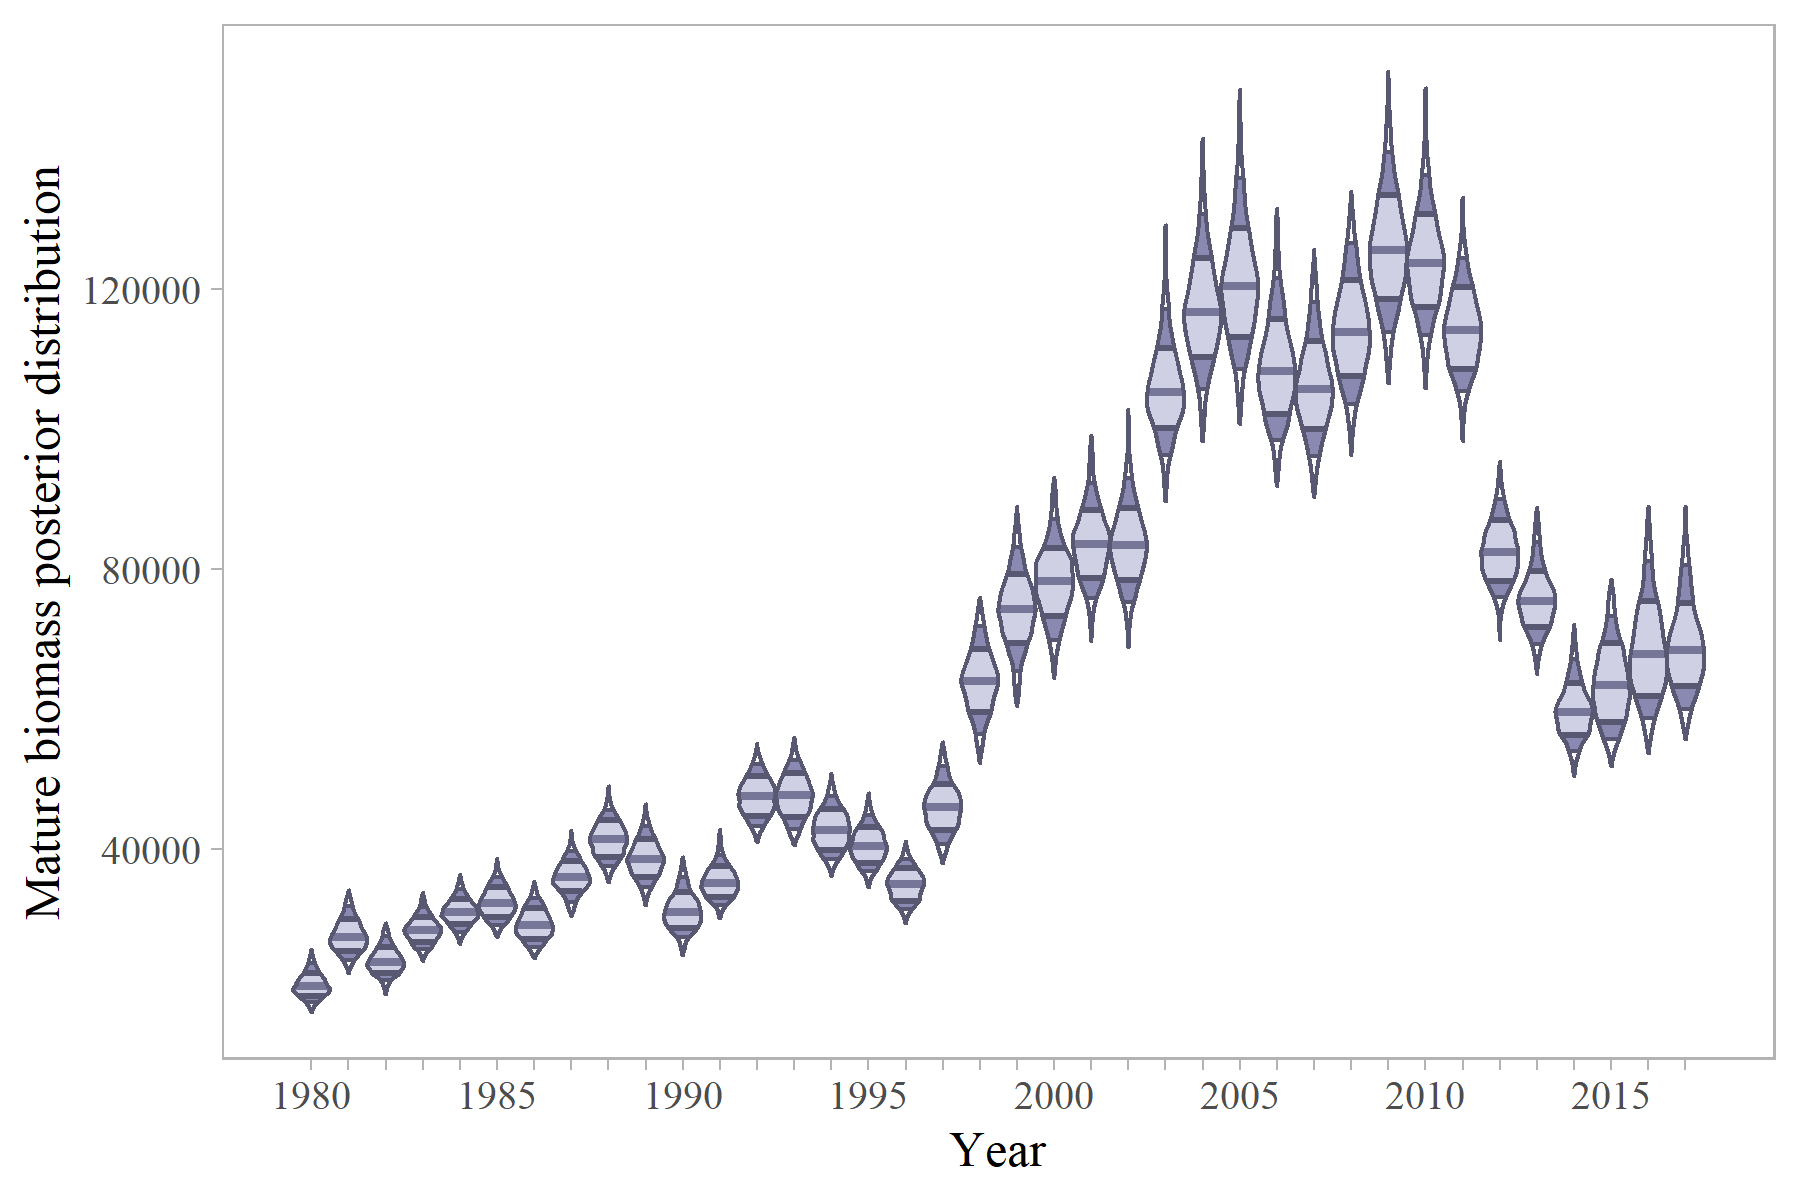
\includegraphics[width=1\linewidth]{../../HER/figs/HER/posterior_matbiomass}

Figure 23. The full posterior densities of mature biomass, including the
median (line) and 50\% (lighter shading) and 95\% percentiles (darker
shading).

We've identified the `adnuts' package, written by Cole Monnahan, a past
UW PhD student, as a viable option for running HER in a Bayesian
framework. The methods and motivation for the `adnuts' package was
published this year in PlosOne and was coauthored by the lead developer
of TMB, Kasper Kristensen (Monnahan and Kristensen 2018). The workhorse
algorithm NUTS (no U-turn sampler) was originally developed by Hoffman
and Gelman (2014).

The `adnuts' package came out of Monnahan's dissertation, which focused
on advancing Bayesian methods in fisheries science (Monnahan 2017).
Traditional MCMC methods when applied to complicated models (i.e., age-
and length-structured stock assessments or hierarchical models) are slow
and inefficient. During the heyday of ADMB, most assessments relied on
frequentist methods for inference. Consequently ADMB's existing
infrastructure for implementing Bayesian methods is pretty rudimentary.
In Monnahan's second chapter, he tested the existing Bayesian algorithms
compared to NUTS for 6 stock assessment models and found NUTS to be
faster (10-1000x) and more reliable at fully exploring posterior
parameter space.

Benefits of the `adnuts' package include: 1) the framework, functions,
and capabilities are similar to what is contemporaneously used for TMB
and STAN models; and 2) early explorations suggest that it greatly
increases our ability to do MCMC sampling via multiple choices for
algorithms, the ability to execute multiple chains (oddly not a built-in
feature in ADMB), built-in diagnostic features, and the choice to change
starting values (ADMB defaults to MLE estimates, which can be
problematic if converging at a local minima). There are also other bells
and whistles like the ability to run chains on multiple cores and an
argument for setting time duration that will stop sampling after the set
time (especially useful for model testing and running your model
overnight).

\subsection{Next steps}\label{next-steps-2}

While the posterior samples are written, more code should be developed
for diagnostic plots and visualizing variance estimation.

During review, it was discussed that there were marked differences in
the estimated variance of maturity and selectivity. Potential reasons
for this include 1) the small time period defined for the second
maturity time block, 2) the rescaling of selectivity (Jane examined this
and it was not the case), 3) the model is conditioned on catch (perhaps
if it was conditioned on effort selectivity would be more variable), and
4) the population dynamics equations are currently written such that
catch is not assumed to be 100\% mature as in the LS model (thus
resulting in additional variability in maturity).

It was discussed that the variability on forecasted spawning stock
biomass was very narrow. It is unclear why this is the case, but should
be examined more in the future.

Sherri and Sara wanted the age-3 abundance as estimated by the ASA
model, instead of recruitment as estimated by the Ricker curve, which is
how the tpl is currently coded. This can be easily corrected in future
developments.

Finally future development should include running the MCMC evaluation
using functions from the `adnuts' library, so that we can test different
starting values, run the model with multiple chains, test the efficiency
of the alternative NUT algorithm, and utilize the more comprehensive
built-in suite of diagnostic tools. Additionally, we currently estimate
variance on maturity and selelctivity-at-age (or estimated recruitment),
but do not run the MCMC on the actual parameters for the logistic or
Ricker curves. It would be a good next step to complete this task and
explore correlations between these parameters.

\section{HER retrospective behavior}\label{her-retrospective-behavior}

The corresponding code for the retrospective analysis is found in
R/retrospective.R

Definitions:

\emph{Terminal year} - the most recent year of the assessment

\emph{Peel} - removing a year and re-running the most current assessment
for that year

The figure generated for the retrospective analysis shows retrospective
behavior of spawning biomass and the percent difference from the
terminal year for each peel (Figure 24). These figures were modeled
after figures presented at a workshop of the Alaska Groundfish Plan
Teams (Clark et al 2012).

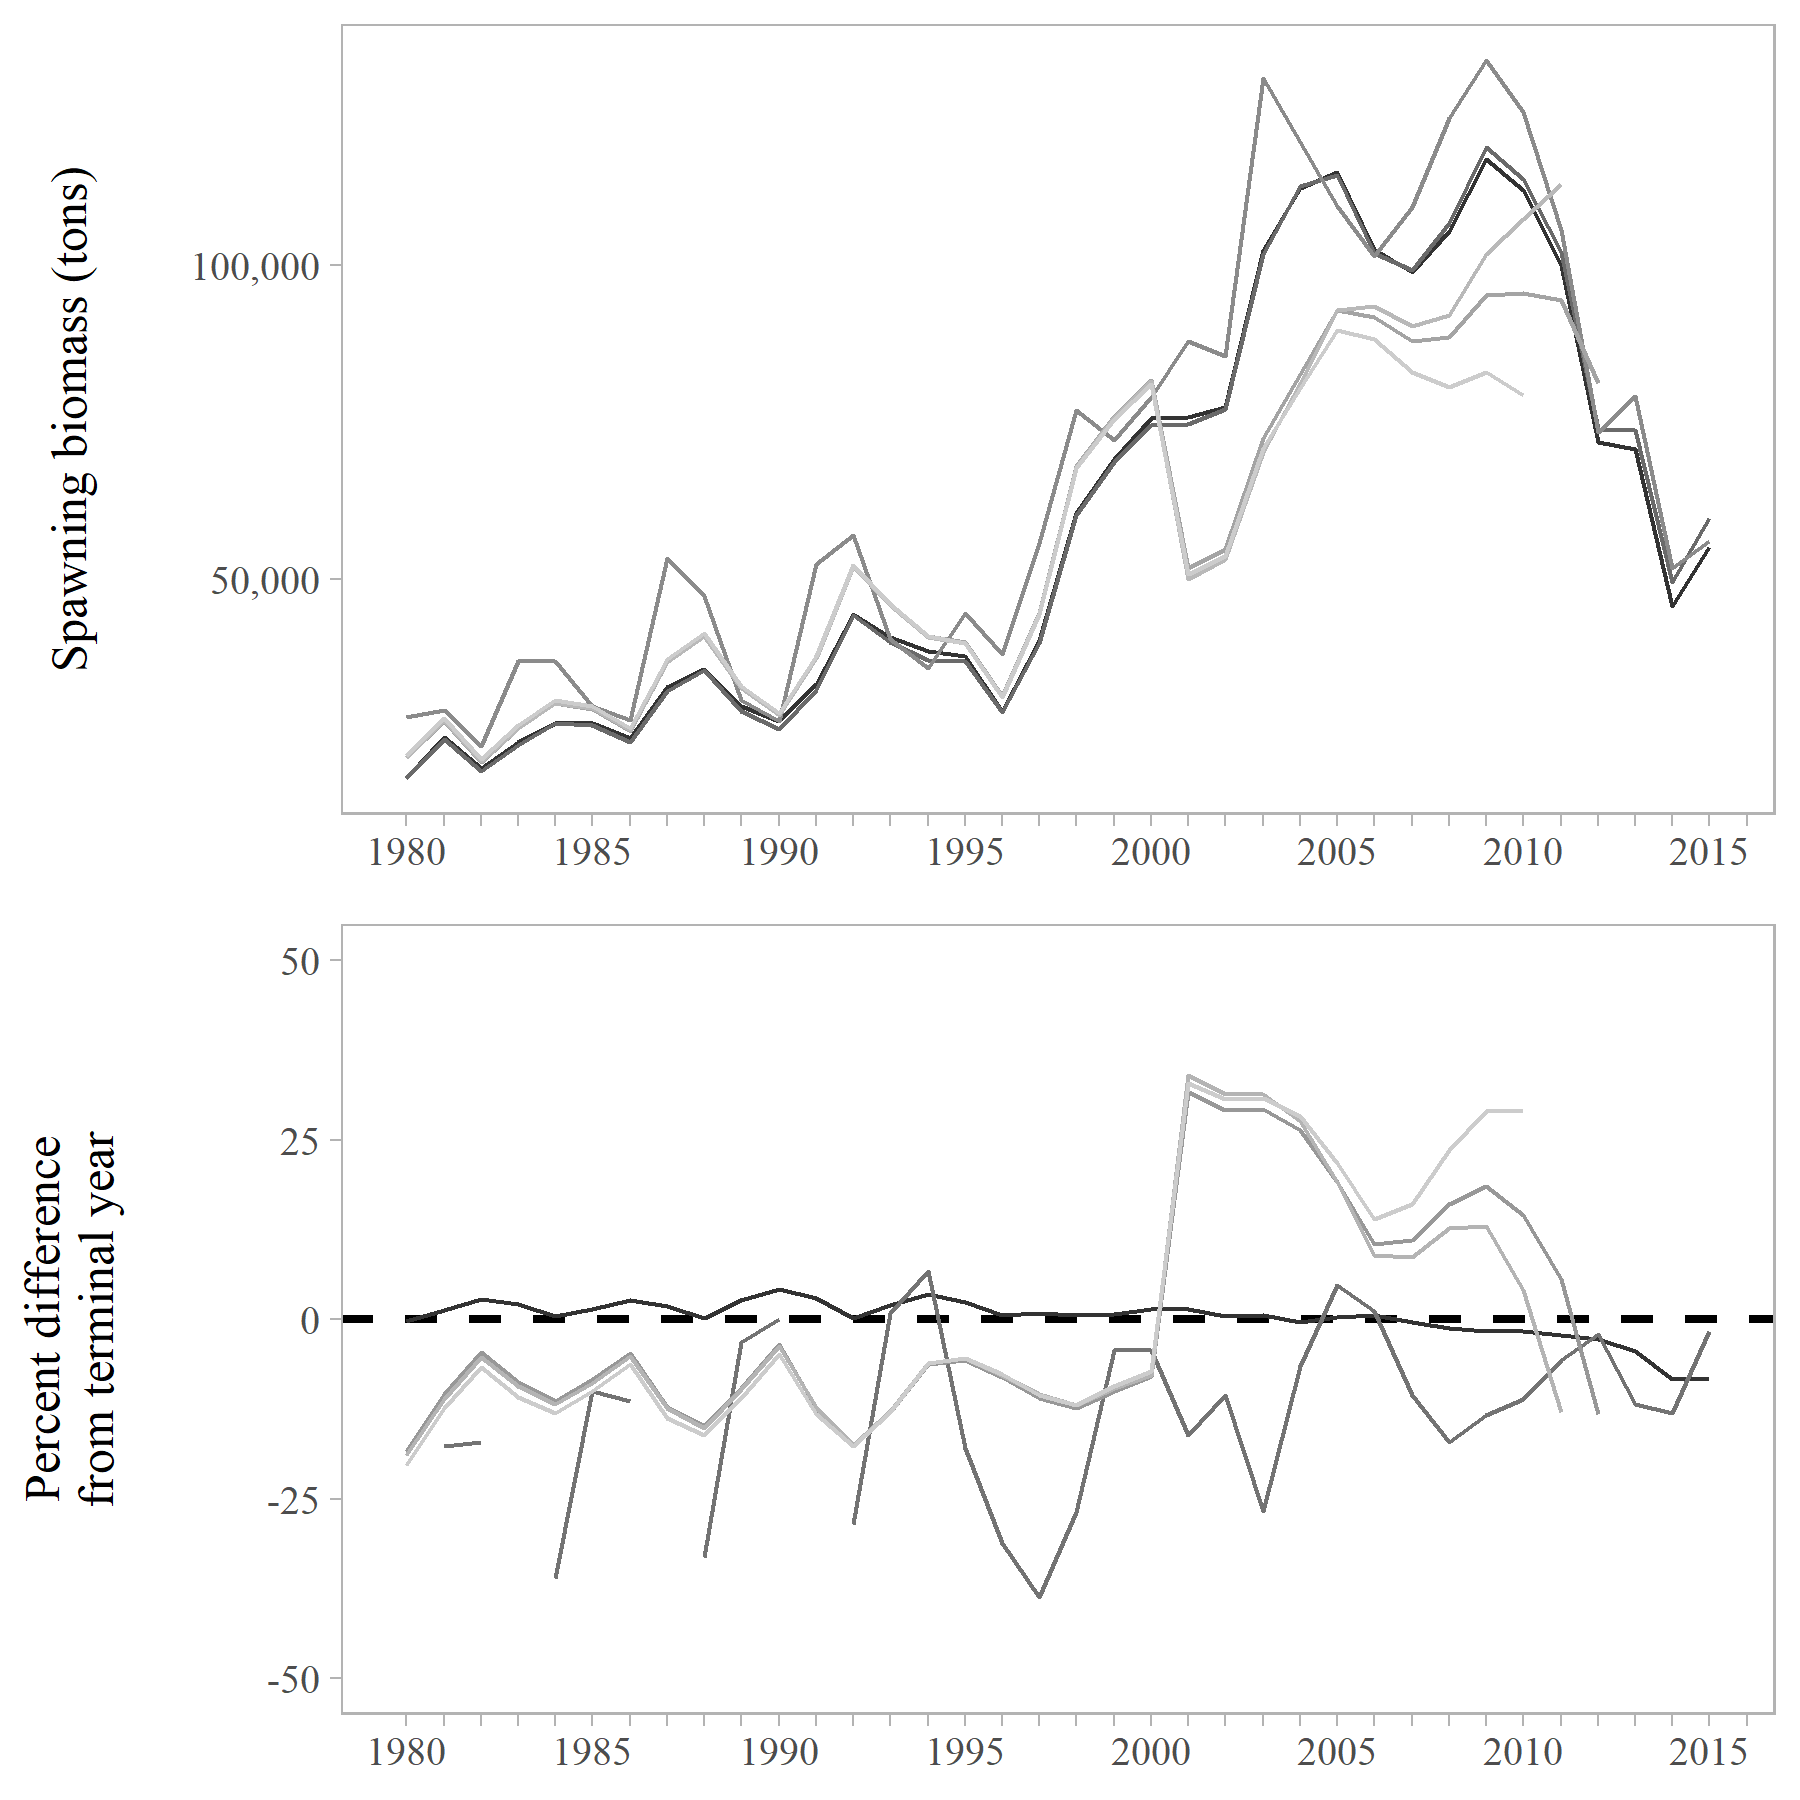
\includegraphics[width=1\linewidth]{../../HER/figs/HER/retrospective}

Figure 24. Retrospective analysis of HER estimates of spawning stock
biomass (tons) on the top, and the percent difference of each peel from
the terminal year on the bottom

Two summary statistics are calculated: the first is the Mohn's Rho as
defined by the Alaska Fisheries Science Center and Hurtado-Ferro et al.
(2015), which is the difference between the estimate in a peel year and
the reference estimate from the terminal year divided by the reference
estimate and summed across all peels. The second statistic, the Wood's
Hole Rho, uses all estimates in the peel, not just the final estimate.
LeGault et al. (2009) found no marked differences between the two rhos.
These statistics are written to a file called
`HER/retrospective\_rhos.csv'. Mohn's and Wood's Rhos were quite small
for this version of the model (0.08 and -0.005, respectively).

An excerpt from Hurtado-Ferro et al. (2015) regarding the interpretation
of Mohn's Rho: Given that the variability of Mohn's rho depends on life
history, and that the statistic appears insensitive to F, we propose the
following rule of thumb when determining whether a retrospective pattern
should be addressed explicitly: values of Mohn's r higher than 0.20 or
lower than 20.15 for longer-lived species (upper and lower bounds of the
90\% simulation intervals for the flatfish base case), or higher than
0.30 or lower than 20.22 for shorter-lived species (upper and lower
bounds of the 90\% simulation intervals for the sardine base case)
should be cause for concern and taken as indicators of retrospective
patterns. However, Mohn's Rho values smaller than those proposed should
not be taken as confirmation that a given assessment does not present a
retrospective pattern, and the choice of 90\% means that a ``false
positive'' will arise 10\% of the time.

Because the version of HER presented in this document has time blocks
for maturity and natural mortality starting in 2015, the current
retrospective code will not run for all peels (it runs for the first 2,
then stops). In order to accomodate this issue and provide an example of
a working retrospective analysis for HER, I created a new branch called
`retrospective' in the AlaskaHerring repository, and made the following
changes to the HER/sitka\_2.ctl file:

Maturity blocks: 1980-1998 and 1999-2017 Natural mortality blocks:
1980-1998 and 1999-2017

It ran successfully for 7 peels, and I ran into non-convergence on the
8th peel. In addition to summarizing r

\subsection{Next steps}\label{next-steps-3}

I recommend two steps forward on the retrospective analysis for HER. The
first is to modify the read\_admb() function to better accomodate runs
that do not converge. Currently I get an error ``Error in
file(con,''r``) : cannot open the connection In addition: Warning
message: In file(con,''r``) : Error in file(con,''r``) : cannot open the
connection. I do not fully understand this error but know it traces back
to the read\_fit() function that is nested inside the read\_admb()
function.

The second recommendation is to figure out a solution for dealing with
peels that go beyond a break in a time block for a time-varying
parameter. This could be something to bring up during Punt's course, to
Steve Martell, or perhaps at Groundfish Plan Team.

\section{HER simulation}\label{her-simulation}

The simulation approach used is called ``self-testing,'' where the same
model (with known parameters) is used to generate data and then estimate
parameters based on the simulated data. This approach should generate
exact parameter estimates in the case where data are generated with no
simulated observation errors. The step-by-step code and documentation is
written in R/simulations.R. Currently it is written to condition/fit the
model to the Sitka data then use these parameter values to estimate data
and then re-estimate parameters. Currently the simulation self-tests
perfectly, but does not include any observation or process error. This
would be a future development and perhaps something to ask S. Martell
about.

\subsection{Next steps}\label{next-steps-4}

Sherri and I discussed that this as an area for considerable development
and may be a potential contract with Steve Martell.

\section{Likelihood profiles}\label{likelihood-profiles}

The motivation for examining likelihood profiles, which are the minimum
negative log-likelihoods for a range of values of a single parameter, is
generally two-fold: 1) calculating confidence intervals, and 2)
examining properties of the likelihood surface
(e.g.~smoothness/steepness of the parameter space, presence of local
minima, etc.). In Bayesian analyses, both of these are replaced by
examining the posterior distribution.

The standard ADMB procedure for calculating likelihood profiles is
proving very difficult to apply to HER. According to Ben Bolker's
chapter on likelihood, specifically pages 31-35, it's not surprising
that I'm encountering difficulty estimating likelihood profile surfaces
for such a complex model. He points out that likelihood profiles are not
used for variance estimation of such complex models, and that instead
the second derivatives of the log-likelihood as a function of the
parameters (aka the Hessian matrix) are used. From here the Hessian, the
`negative of the expected value' of the Hessian (the Fisher information
matrix), and the `Fisher evaluated at the maximum likelihood estimate'
(the observed information matrix) represent the curvature of the
likelihood surface along a particular axis. This will tell us everything
we need to know about model fit and uncertainty. Perhaps in Andre's
course we will learn more about how to utilize the Hessian to explore
parameter space, but at the moment I feel ill-equipped to venture out
into the Hessian, the Fisher information, or the observed information
matrix alone. I think instead that an examination of the posteriors will
give us all the information we need to know.

\subsection{Next steps}\label{next-steps-5}

The topics of exploring likelihood profiles is something Sherri would
like me to pursue during Punt's course.

\section{References}\label{references}

Clark, B., D. Hanselman, M. Sigler. 2012. Report of the retrospective
analysis working group. September 2012 Plan Team Draft.
\url{https://www.afsc.noaa.gov/refm/stocks/plan_team/2012/sept/retrospective_analysis.pdf}

Hoffman, M.D.~and Gelman, A. 2014. The No-U-turn sampler: adaptively
setting path lengths in Hamiltonian Monte Carlo. Journal of Machine
Learning Research, 15(1), pp.1593-1623.

Hulson, P.F., Quinn II, T.J., Dressel, S.C. 2014. Description and
improvement of the age-structured assessment model for Pacific herring
in Sitka Sound, Alaska. DRAFT.

Hurtado-Ferro, F., Szuwalski, C. S., Valero, J. L., Anderson, S. C.,
Cunningham, C. J., Johnson, K. F., Licandeo, R., McGilliard, C. R.,
Monnahan, C. C., Muradian, M. L., Ono, K., Vert-Pre, K. A., Whitten, A.
R., and Punt, A. E. Looking in the rear-view mirror: bias and
retrospective patterns in integrated, age-structured stock assessment
models. 2015. ICES Journal of Marine Science, 72(1), 99--110.
\url{doi:10.1093/icesjms/fsu198}

Legault, C.M., Chair. 2009. Report of the Retrospective Working Group,
January 14-16, 2008, Woods Hole, Massachusetts. US Dept Commer,
Northeast Fish Sci Cent Ref Doc. 09-01; 30 p.~Available from: National
Marine Fisheries Service, 166 Water Street, Woods Hole, MA 02543-1026,
or online at \url{http://www.nefsc.noaa.gov/nefsc/publications/}

Monnahan, C., 2017. Advancing Bayesian methods in fisheries stock
assessment (Doctoral dissertation). University of Washington.
\url{https://digital.lib.washington.edu/researchworks/bitstream/handle/1773/40702/Monnahan_washington_0250E_17687.pdf?sequence=1}

Martell, S.J.D. 2016. Age-structured model for Alaska herring stocks.
\url{https://github.com/commfish/AlaskaHerring/blob/master/docs/modelDescription/TechnicalDoc.pdf}

Monnahan CC, Kristensen K (2018) No-U-turn sampling for fast Bayesian
inference in ADMB and TMB: Introducing the adnuts and tmbstan R
packages. PLoS ONE 13(5): e0197954.
\url{https://doi.org/10.1371/journal}. pone.0197954

\section{Other lingering questions and future
development}\label{other-lingering-questions-and-future-development}

\begin{itemize}
\item
  What does the value() fxn do and when do you have to use it?
\item
  How do you get likelihood profiles for time-varing parameters?
\item
  If a parameter has both an upper bound and a lower bound, as well as
  parameters for a uniform prior, what are the actual bounds for
  estimation?
\item
  Extracting time varying maturity parameters in report file (currently
  hard-coded so you have to know how many blocks there are ahead of
  time).
\item
  When meeting with Kyle on herring data, review whether or not we want
  to round biomass (significant digits). Look also at other ASA models
  to see if they should be rounded.
\item
  In the Technical Document, Steve indicates that the HER code readily
  provides the means to calculate MSY or SPR-based reference points and
  associated uncertainty, however, there is no mention of this in the
  code itself.
\item
  Revisit the question of how to treat selectivity. Do we apply
  selectivity to numbers-at-age as is done now in both HER and LS, such
  that it is essentially the combination of availability and fishery
  selectivity? Or do we change it so that numbers-at-age is first
  multiplied by maturity and then by selectivity (such that selectivity
  in this case is fishery selectivity alone and maturity deals with the
  fish that are available to the fishery on the spawning grounds)?
\item
  Currently spawner and fishery weight-at-age are identical (fishery is
  used for spawner weight-at-age in all years except 1997) - do we
  really feel like 1997 should be an exception? Also, why do we collect
  cast net weight-at-age if we don't use them? In PWS they take gonad
  condition to determine proportion mature.
\item
  We currently assume the spawning population has a 50:50 sex ratio. Do
  we have data to support this assumption or otherwise?
\end{itemize}


\end{document}
